\documentclass[11pt,a4paper]{article}

% ── Packages ──────────────────────────────────────────────────────────────
\usepackage[utf8]{inputenc}
\usepackage[T1]{fontenc}
\usepackage{lmodern}
\usepackage[margin=2.5cm]{geometry}
\usepackage{amsmath,amssymb,amsthm}
\usepackage{mathtools}
\usepackage{bm}
\usepackage{enumitem}
\usepackage{hyperref}
\usepackage{xcolor}
\usepackage{tcolorbox}
\usepackage{booktabs}
\usepackage{graphicx}
\usepackage{tikz}
\usepackage{tikz-3dplot}
\usetikzlibrary{arrows.meta,calc,decorations.pathreplacing}
\usepackage{fancyhdr}
\usepackage{titlesec}

% ── Colours (from course palette) ────────────────────────────────────────
\definecolor{colspace}{HTML}{3B82F6}
\definecolor{response}{HTML}{F59E0B}
\definecolor{projection}{HTML}{10B981}
\definecolor{residual}{HTML}{EF4444}
\definecolor{constraint}{HTML}{8B5CF6}
\definecolor{secondary}{HTML}{6B7280}

% ── Theorem environments ─────────────────────────────────────────────────
\theoremstyle{plain}
\newtheorem{theorem}{Theorem}[section]
\newtheorem{proposition}[theorem]{Proposition}
\newtheorem{lemma}[theorem]{Lemma}
\newtheorem{corollary}[theorem]{Corollary}

\theoremstyle{definition}
\newtheorem{definition}[theorem]{Definition}
\newtheorem{example}[theorem]{Example}
\newtheorem{remark}[theorem]{Remark}

% ── Custom boxes ─────────────────────────────────────────────────────────
\newtcolorbox{keyinsight}{
  colback=projection!8, colframe=projection!80!black,
  fonttitle=\bfseries, title=Key Geometric Insight,
  arc=2mm, boxrule=0.8pt
}

\newtcolorbox{warning}{
  colback=residual!8, colframe=residual!80!black,
  fonttitle=\bfseries, title=Warning,
  arc=2mm, boxrule=0.8pt
}

\newtcolorbox{metaphor}{
  colback=response!8, colframe=response!80!black,
  fonttitle=\bfseries, title=The Flashlight Metaphor,
  arc=2mm, boxrule=0.8pt
}

% OP-0.1: Stop-and-Think and Misconception box definitions
\newtcolorbox{stopandthink}{
  colback=colspace!8, colframe=colspace!80!black,
  fonttitle=\bfseries, title={\raisebox{-0.1em}{\Large ?}\;\;Stop and Think},
  arc=2mm, boxrule=0.8pt
}

\newtcolorbox{misconception}{
  colback=residual!8, colframe=residual!80!black,
  fonttitle=\bfseries, title={Misconception Alert},
  arc=2mm, boxrule=0.8pt
}

% ── Header / footer ──────────────────────────────────────────────────────
\pagestyle{fancy}
\fancyhf{}
\fancyhead[L]{\small\textsc{The Geometry of Linear Regression}}
\fancyhead[R]{\small\thepage}
\renewcommand{\headrulewidth}{0.4pt}

% ── Macros ────────────────────────────────────────────────────────────────
\newcommand{\R}{\mathbb{R}}
\newcommand{\yhat}{\hat{\bm{y}}}
\newcommand{\bhat}{\hat{\bm{\beta}}}
\newcommand{\btilde}{\tilde{\bm{\beta}}}
\newcommand{\bX}{\bm{X}}
\newcommand{\by}{\bm{y}}
\newcommand{\be}{\bm{e}}
\newcommand{\bH}{\bm{H}}
\newcommand{\bM}{\bm{M}}
\newcommand{\bI}{\bm{I}}
\newcommand{\bQ}{\bm{Q}}
\newcommand{\bD}{\bm{D}}
\newcommand{\Col}{\mathcal{C}}
\newcommand{\ip}[2]{\langle #1, #2 \rangle}
\newcommand{\norm}[1]{\left\lVert #1 \right\rVert}
\DeclareMathOperator{\tr}{tr}
\DeclareMathOperator{\rank}{rank}
\DeclareMathOperator{\diag}{diag}
\DeclareMathOperator*{\argmin}{arg\,min}

% ── Title (OP-13.4: subtitle added) ─────────────────────────────────────
\title{%
  \textbf{The Geometry of Linear Regression}\\[6pt]
  \large Lecture Notes: Seeing OLS Through the Projection Theorem\\[4pt]
  \vspace{0.5em}{\large\itshape Supplementary notes for the lecture on linear regression}
}
\author{Statistical Machine Learning Lab}
\date{Spring 2026}

\begin{document}
\maketitle
\thispagestyle{fancy}

\begin{abstract}
These lecture notes develop ordinary least squares (OLS) regression entirely
from the perspective of the \emph{Projection Theorem} in inner product spaces.
Every classical result---the normal equations, variance decomposition,
$R^2$, the Gauss--Markov theorem, the Frisch--Waugh--Lovell theorem,
leverage and influence diagnostics, multicollinearity, omitted variable
bias, Ridge and LASSO regularisation, the $F$-test, and confidence
ellipsoids---is derived as a geometric consequence of orthogonal
projection onto the column space of the design matrix.
The unifying principle: \emph{regression is a shadow cast by the data vector
onto the column space, and the residual is the perpendicular distance from
object to shadow.}
\end{abstract}

\tableofcontents
\newpage

%======================================================================
% OP-1.1: REPLACE prologue with round3 revised prologue
%======================================================================
\section{Prologue: One Theorem, Ten Perspectives}
%======================================================================

\subsection*{New Year's Night, 1802}

On the first day of the nineteenth century, the astronomer Giuseppe Piazzi
spotted something that should not have been there: a faint, slow-moving
point of light in the constellation Taurus.  Night after night he tracked
it, recording its position against the fixed stars.  He had discovered
Ceres---the first asteroid, and the largest object between Mars and
Jupiter.

Then disaster struck.  After only 41 nights of observation, Ceres
drifted too close to the Sun and vanished in the glare.
Piazzi had captured barely three percent of the asteroid's orbit.  As the
months passed, the astronomical community faced a crisis: by the
time Ceres emerged from behind the Sun, it could be \emph{anywhere} along
a vast arc of sky.  Several astronomers tried to predict its return,
assuming a circular orbit; their predictions would miss by more than ten
degrees.  The needle had disappeared into a haystack of stars.

A 24-year-old mathematician in Brunswick named Carl Friedrich Gauss
took a different approach.

Gauss took Piazzi's 41 data points---each one contaminated by
atmospheric distortion, instrument imprecision, and the tremor of a
human hand---and asked a question that would reshape the mathematics of
uncertainty: \emph{Of all the elliptical orbits that the laws of physics
permit, which one passes closest to these noisy observations?}

His method was, at its core, simple.  He wrote down the
equations of a Keplerian ellipse, parameterised by six orbital elements.
These equations carved out a surface---a subspace of possible
trajectories---inside the much larger space of all conceivable sequences
of celestial positions.  Piazzi's 41 observations lived somewhere in that
larger space, displaced from the true orbit by the accumulated noise of
every measurement.  Gauss sought the single point on the orbital surface
that lay \emph{nearest} to the data.

He found it by dropping a perpendicular.

The computation was ferocious: weeks of hand calculation, pages of
logarithm tables, corrections for the Sun's gravitational tug.  But the
geometric principle was clear.  The best-fitting orbit was the
\textbf{shadow} of the noisy data cast onto the subspace of physically
possible trajectories---the point where a perpendicular from the data
meets the surface.  The residual---the gap between data and
prediction---stood at a right angle to every direction the orbit could
vary.  Gauss kept his method private; only years later would it become
known as the \emph{method of least squares}.

Gauss sent his prediction to the astronomer Franz Xaver von Zach.  On
December~31, 1801---New Year's Eve---von~Zach aimed his telescope at the
patch of sky Gauss had specified.  There, within half a degree of the
predicted position, was Ceres.

It was one of the greatest predictions in the history of science.
And it was, at its mathematical heart, an orthogonal projection.

\bigskip

\subsection*{From the stars to the spreadsheet}

Two centuries later, the same geometry appears every time you fit a
model to data.  The setting is humbler---you might be predicting house
prices instead of asteroid trajectories---but the underlying act is
identical.  Your data vector $\by\in\R^n$ lives in a high-dimensional
space.  The column space of your design matrix $\Col(\bX)$ is a subspace
of possible fitted values, one for each choice of coefficients.  The
ordinary least squares fit $\yhat$ is the point in $\Col(\bX)$ closest
to $\by$.  The residual $\be = \by - \yhat$ is perpendicular to the
column space.

Gauss projected noisy observations onto the subspace of Keplerian
ellipses.  You project noisy responses onto the subspace spanned by
your regressors.  The theorem that makes both possible is the same.

\begin{metaphor}
Imagine a flashlight shining straight down onto a table.
The \textbf{object} is the data vector $\by\in\R^n$, hovering above.
The \textbf{table} is the column space $\Col(\bX)$.
The \textbf{shadow} on the table is the fitted vector $\yhat$.
The \textbf{gap} between object and shadow is the residual $\be$.
The shadow falls directly below---the residual is
perpendicular to the table.
\end{metaphor}

This single image---a shadow cast at right angles---generates everything
in these notes.

% OP-1.2: INSERT Figure 1 (flashlight metaphor)
\begin{figure}[ht]
\centering
\tdplotsetmaincoords{70}{120}
\begin{tikzpicture}[tdplot_main_coords, scale=1.6, >=Stealth]

  % --- Ground plane Col(X) ---
  \fill[colspace!12] (-2.8,-2.8,0) -- (2.8,-2.8,0) -- (2.8,2.8,0) -- (-2.8,2.8,0) -- cycle;
  \draw[colspace!40] (-2.8,-2.8,0) -- (2.8,-2.8,0) -- (2.8,2.8,0) -- (-2.8,2.8,0) -- cycle;
  \node[colspace!80!black, font=\footnotesize\itshape] at (2.2,-2.2,0) {$\operatorname{Col}(\bm{X})$};

  % --- Flashlight (cone of light from above) ---
  \coordinate (lamp) at (0.8,0.3,4.5);
  % Light cone: four semi-transparent rays
  \foreach \dx/\dy in {-0.6/-0.6, 0.6/-0.6, 0.6/0.6, -0.6/0.6}{
    \draw[response!30, line width=0.4pt] (lamp) -- ($(0.8,0.3,0)+(\dx,\dy,0)$);
  }
  % Filled cone hint
  \fill[response!8] (lamp) -- (0.2,-0.3,0) -- (1.4,-0.3,0) -- (1.4,0.9,0) -- (0.2,0.9,0) -- cycle;

  % Flashlight body
  \shade[ball color=secondary!60] (lamp) circle (3pt);
  \node[above, secondary, font=\footnotesize] at (lamp) {flashlight};

  % --- Object y floating above the plane ---
  \coordinate (ypos) at (0.8, 0.3, 2.6);
  \shade[ball color=response!80] (ypos) circle (3.5pt);
  \node[right=4pt, response!80!black, font=\bfseries] at (ypos) {$\bm{y}$};

  % --- Shadow yhat on the plane ---
  \coordinate (yhat) at (0.8, 0.3, 0);
  \shade[ball color=projection!80] (yhat) circle (3.5pt);
  \node[below right=2pt, projection!80!black, font=\bfseries] at (yhat) {$\hat{\bm{y}}$};

  % --- Residual: dashed vertical line y -> yhat ---
  \draw[residual, thick, dashed] (ypos) -- (yhat);
  \node[left=3pt, residual!80!black, font=\footnotesize\bfseries] at ($(ypos)!0.5!(yhat)$) {$\bm{e}$};

  % --- Right-angle mark at yhat ---
  \draw[secondary, line width=0.6pt]
    ($(yhat)+(0,0.18,0)$) -- ($(yhat)+(0,0.18,0.18)$) -- ($(yhat)+(0,0,0.18)$);

\end{tikzpicture}
\caption{The flashlight metaphor.  Think of the data vector~$\bm{y}$ as an
object suspended above the column space of~$\bm{X}$.  A flashlight shining
straight down casts a \emph{shadow}~$\hat{\bm{y}}$ on the plane.  The
vertical gap between object and shadow is the residual~$\bm{e}$, and it
meets the plane at a right angle --- exactly as orthogonal projection
demands.}
\label{fig:flashlight}
\end{figure}

\begin{theorem}[The Projection Theorem---finite-dimensional case]%
  \label{thm:projection}
Let $S$ be a subspace of $\R^n$, and let $\by\in \R^n$.  There exists
a unique $\yhat\in S$ such that
\[
  \norm{\by - \yhat} \;\le\; \norm{\by - \bm{s}}
  \qquad\text{for all } \bm{s}\in S.
\]
Moreover, $\yhat$ is characterised by the \emph{orthogonality condition}
\[
  (\by - \yhat) \perp S,
\]
i.e.\ $\ip{\by - \yhat}{\bm{s}} = 0$ for every $\bm{s}\in S$.
\end{theorem}

Ordinary least squares is the Projection Theorem applied to
$S = \Col(\bX)$.
That one sentence is the seed from which the rest of these notes grow.

\subsection*{Roadmap}

Every section that follows answers a question that the Projection
Theorem makes natural:

% OP-1.1 modification: strip roadmap to questions only (no geometric-insight spoilers)
\begin{enumerate}[leftmargin=2em]
  \item \textbf{Where do the coefficients come from?}
    (\S\ref{sec:coefficients})

  \item \textbf{How good is the fit?}
    (\S\ref{sec:pythagoras})

  \item \textbf{What does each variable contribute on its own?}
    (\S\ref{sec:fwl})

  \item \textbf{What can go wrong, and how do we fix it?}
    (\S\ref{sec:leverage}--\S\ref{sec:regularisation})

  \item \textbf{How do we test whether the shadow is real?}
    (\S\ref{sec:ftest})
\end{enumerate}

\noindent
By the time you reach the end, you will see that Gauss's prediction of
Ceres, the $R^2$ on your next problem set, and the $p$-value in a
clinical trial are all manifestations of the same geometric act:
dropping a perpendicular onto a subspace, and measuring the gap that
remains.

% OP-1.3: INSERT transition sentence (Prologue -> Section 2)
\medskip
\noindent\textit{The Projection Theorem guarantees that a closest point
exists and is characterised by orthogonality.
But how do we actually \emph{compute} it?
The next section translates the geometric existence result into an
explicit formula---the normal equations---and shows that the OLS
coefficients are simply the coordinates of this closest point.}

% OP-1.4: INSERT Stop-and-Think 1
\begin{stopandthink}
\textbf{Exercise.}
Take $\by = (3, 1)^\top$ and $\bm{x} = (2, 1)^\top$ in $\R^2$.
The column space $\Col(\bm{x})$ is the line through the origin in the
direction $(2,1)$.
\begin{enumerate}[nosep]
  \item Sketch the vectors $\by$ and $\bm{x}$ in $\R^2$.
  \item Compute the projection of $\by$ onto $\Col(\bm{x})$ using the
        formula $\yhat = \bm{x}(\bm{x}^\top\bm{x})^{-1}\bm{x}^\top\by$.
        Where does the projection land on the line?
  \item Draw the residual vector $\be = \by - \yhat$.
        Verify visually that it is perpendicular to $\bm{x}$.
  \item Compute $\bm{x}^\top \be$ and confirm it equals zero.
\end{enumerate}
\emph{Answer check:} You should get $\yhat = \tfrac{7}{5}(2, 1)^\top
= (2.8,\, 1.4)^\top$ and $\be = (0.2,\, -0.4)^\top$.
\end{stopandthink}


%======================================================================
\section{Where Coefficients Come From}\label{sec:coefficients}
%======================================================================

% OP-2.1: INSERT Standing Assumption box
\begin{tcolorbox}[
  colback=colspace!8, colframe=colspace!80!black,
  fonttitle=\bfseries, title=Standing Assumption,
  arc=2mm, boxrule=0.8pt
]
\textbf{Full column rank.}
Throughout these notes (unless stated otherwise), we assume that the
$n\times p$ design matrix $\bX$ has \textbf{full column rank}:
$\rank(\bX) = p$, with $n \ge p$.

This is equivalent to any of the following:
\begin{enumerate}[nosep,label=(\roman*)]
  \item The columns of $\bX$ are linearly independent.
  \item The Gram matrix $\bX^\top\bX\in\R^{p\times p}$ is invertible
        (positive definite).
  \item The column space $\Col(\bX)$ has dimension exactly $p$.
  \item No predictor is an exact linear combination of the others.
\end{enumerate}
Without this assumption, $(\bX^\top\bX)^{-1}$ does not exist, and the OLS
coefficient vector $\bhat$ is not uniquely determined (although the
fitted values $\yhat = \bH\by$ remain unique as a projection).
\end{tcolorbox}

\subsection{Setup and notation}

We observe $n$ data points $(x_i, y_i)$, $i=1,\dots,n$.
Stack the responses into a single vector
$\by = (y_1,\dots,y_n)^\top \in \R^n$ and form the
$n\times p$ \textbf{design matrix}
\[
  \bX = \begin{pmatrix} \bm{x}_1^\top \\ \vdots \\ \bm{x}_n^\top \end{pmatrix}
  \in \R^{n\times p},
\]
where typically the first column is a column of ones (the intercept).
The \textbf{column space} of $\bX$ is
\[
  \Col(\bX) = \bigl\{\bX\bm{\beta} : \bm{\beta}\in\R^p\bigr\}
  \;\subseteq\; \R^n.
\]
Every vector in $\Col(\bX)$ represents the set of fitted values for
\emph{some} choice of coefficients.

\subsection{OLS as orthogonal projection}

\begin{definition}[OLS estimator]
The OLS estimator is
\[
  \bhat = \argmin_{\bm{\beta}\in\R^p}
  \norm{\by - \bX\bm{\beta}}^2.
\]
\end{definition}

Since $\Col(\bX)$ is a closed subspace of $\R^n$, the Projection Theorem
(\ref{thm:projection}) guarantees a unique minimiser.
The fitted values $\yhat = \bX\bhat$ are the orthogonal projection of $\by$
onto $\Col(\bX)$, and the residual
$\be = \by - \yhat$
is perpendicular to $\Col(\bX)$.

\begin{keyinsight}
$\bhat$ is the coordinate vector of the foot of the perpendicular
from $\by$ to $\Col(\bX)$.
The coefficients are not arbitrary numbers from a formula---they locate
the point on the column space closest to the data.
\end{keyinsight}

\subsection{The normal equations}

The orthogonality condition $\be \perp \Col(\bX)$ means
$\ip{\bX\bm{v}}{\be} = 0$ for all $\bm{v}\in\R^p$, i.e.\
\[
  \bX^\top \be = \bm{0}
  \qquad\Longleftrightarrow\qquad
  \bX^\top(\by - \bX\bhat) = \bm{0}
  \qquad\Longleftrightarrow\qquad
  \boxed{\bX^\top\bX\,\bhat = \bX^\top\by.}
\]
These are the \textbf{normal equations}. If $\bX$ has full column rank,
$\bX^\top\bX$ is invertible and
\begin{equation}\label{eq:ols}
  \bhat = (\bX^\top\bX)^{-1}\bX^\top\by.
\end{equation}
The formula is a recipe for dropping a perpendicular.

\subsection{Building intuition: from $\R^2$ to $\R^n$}

\begin{itemize}[nosep]
\item With $n=2$ observations, $\by\in\R^2$ and the column space is a line
      through the origin (for simple regression with intercept, a line in the plane).
\item With $n=3$, $\by\in\R^3$ and a model with intercept and one predictor
      spans a 2-dimensional plane---the geometry is fully visible.
\item For $n=2000$, the geometry is identical; only the ambient dimension changes.
      The right angle between $\be$ and $\Col(\bX)$ holds in every dimension.
\end{itemize}

% OP-2.2: INSERT Example 1 (shortened -- Step 5 / H^2 verification deleted)
\begin{example}[Your First Regression in $\R^3$]\label{ex:first-regression}
We have $n=3$ observations with one predictor $x$ and a response $y$:
\[
\begin{array}{c|cc}
i & x_i & y_i \\\hline
1 & 1 & 1 \\
2 & 2 & 3 \\
3 & 3 & 2
\end{array}
\]
The model is $y_i = \beta_0 + \beta_1 x_i + e_i$, so the design matrix and response vector are
\[
\bX = \begin{pmatrix} 1 & 1 \\ 1 & 2 \\ 1 & 3 \end{pmatrix}, \qquad
\by = \begin{pmatrix} 1 \\ 3 \\ 2 \end{pmatrix}.
\]
Since $\by\in\R^3$ and $\Col(\bX)$ is a 2-dimensional plane in $\R^3$,
this is literally a point--plane--shadow problem.

\medskip\noindent\textbf{Step 1: Compute $\bX^\top\bX$ and $\bX^\top\by$.}
\[
\bX^\top\bX
= \begin{pmatrix} 1 & 1 & 1 \\ 1 & 2 & 3 \end{pmatrix}
  \begin{pmatrix} 1 & 1 \\ 1 & 2 \\ 1 & 3 \end{pmatrix}
= \begin{pmatrix} 3 & 6 \\ 6 & 14 \end{pmatrix},
\qquad
\bX^\top\by
= \begin{pmatrix} 1 & 1 & 1 \\ 1 & 2 & 3 \end{pmatrix}
  \begin{pmatrix} 1 \\ 3 \\ 2 \end{pmatrix}
= \begin{pmatrix} 6 \\ 13 \end{pmatrix}.
\]

\medskip\noindent\textbf{Step 2: Solve $\bX^\top\bX\,\bhat = \bX^\top\by$.}

The determinant is $\det(\bX^\top\bX) = 3\cdot 14 - 6\cdot 6 = 42 - 36 = 6$, so
\[
(\bX^\top\bX)^{-1}
= \frac{1}{6}\begin{pmatrix} 14 & -6 \\ -6 & 3 \end{pmatrix}
= \begin{pmatrix} 7/3 & -1 \\ -1 & 1/2 \end{pmatrix}.
\]
Therefore
\[
\bhat = (\bX^\top\bX)^{-1}\bX^\top\by
= \begin{pmatrix} 7/3 & -1 \\ -1 & 1/2 \end{pmatrix}
  \begin{pmatrix} 6 \\ 13 \end{pmatrix}
= \begin{pmatrix} 14 - 13 \\ -6 + 13/2 \end{pmatrix}
= \begin{pmatrix} 1 \\ 1/2 \end{pmatrix}.
\]
The fitted line is $\hat{y} = 1 + \tfrac{1}{2}x$.

\medskip\noindent\textbf{Step 3: Compute $\yhat$ and $\be$.}
\[
\yhat = \bX\bhat
= \begin{pmatrix} 1 & 1 \\ 1 & 2 \\ 1 & 3 \end{pmatrix}
  \begin{pmatrix} 1 \\ 1/2 \end{pmatrix}
= \begin{pmatrix} 3/2 \\ 2 \\ 5/2 \end{pmatrix}, \qquad
\be = \by - \yhat
= \begin{pmatrix} 1 \\ 3 \\ 2 \end{pmatrix} - \begin{pmatrix} 3/2 \\ 2 \\ 5/2 \end{pmatrix}
= \begin{pmatrix} -1/2 \\ 1 \\ -1/2 \end{pmatrix}.
\]

\medskip\noindent\textbf{Step 4: Verify the right angle ($\bX^\top\be = \bm{0}$).}
\[
\bX^\top\be
= \begin{pmatrix} 1 & 1 & 1 \\ 1 & 2 & 3 \end{pmatrix}
  \begin{pmatrix} -1/2 \\ 1 \\ -1/2 \end{pmatrix}
= \begin{pmatrix} -1/2 + 1 - 1/2 \\ -1/2 + 2 - 3/2 \end{pmatrix}
= \begin{pmatrix} 0 \\ 0 \end{pmatrix}. \;\checkmark
\]
The residual vector is perpendicular to \emph{every} column of $\bX$,
hence perpendicular to the entire column space---exactly as the
Projection Theorem demands.

\medskip\noindent\textbf{The geometry.}
The data vector $\by = (1, 3, 2)^\top$ is a point in $\R^3$.
The column space $\Col(\bX)$ is the plane spanned by $(1,1,1)^\top$ and $(1,2,3)^\top$.
The fitted vector $\yhat = (3/2,\, 2,\, 5/2)^\top$ is the foot of the perpendicular from $\by$ to this plane.
The residual $\be = (-1/2,\, 1,\, -1/2)^\top$ is the perpendicular itself.
We verified that $\be$ is orthogonal to the plane.

\medskip\noindent\textbf{Takeaway.}
OLS literally drops a perpendicular from $\by$ to $\Col(\bX)$;
the normal equations $\bX^\top\be=\bm{0}$ are the \emph{right-angle condition},
and the hat matrix is the machine that does it.
\end{example}

% OP-2.3: INSERT Figure 2 (Projection in R^3)
\begin{figure}[ht]
\centering
\tdplotsetmaincoords{65}{125}
\begin{tikzpicture}[tdplot_main_coords, scale=1.5, >=Stealth]

  % --- Plane Col(X) through origin ---
  \fill[colspace!10] (-3,-2.5,0) -- (3,-2.5,0) -- (3,2.5,0) -- (-3,2.5,0) -- cycle;
  \draw[colspace!35, line width=0.5pt]
    (-3,-2.5,0) -- (3,-2.5,0) -- (3,2.5,0) -- (-3,2.5,0) -- cycle;
  \node[colspace!80!black, font=\footnotesize\itshape] at (2.5,-2.0,0)
    {$\operatorname{Col}(\bm{X})$};

  % --- Origin ---
  \fill[secondary] (0,0,0) circle (1.5pt);
  \node[below left, secondary, font=\scriptsize] at (0,0,0) {$\bm{0}$};

  % --- Column vectors x1, x2 in the plane ---
  \draw[->, colspace, very thick] (0,0,0) -- (2.4,0.6,0)
    node[right, font=\footnotesize\bfseries] {$\bm{x}_1$};
  \draw[->, colspace!70!black, very thick] (0,0,0) -- (0.8,2.2,0)
    node[above, font=\footnotesize\bfseries] {$\bm{x}_2$};

  % --- Projection yhat ---
  \coordinate (yhat) at (1.8,1.4,0);
  \draw[->, projection, very thick] (0,0,0) -- (yhat)
    node[below right=1pt, font=\footnotesize\bfseries] {$\hat{\bm{y}}$};

  % --- Data vector y above the plane ---
  \coordinate (y) at (1.8,1.4,2.4);
  \draw[->, response, very thick] (0,0,0) -- (y)
    node[above right=1pt, font=\footnotesize\bfseries] {$\bm{y}$};

  % --- Residual e = y - yhat ---
  \draw[->, residual, thick, dashed] (yhat) -- (y)
    node[midway, right=3pt, font=\footnotesize\bfseries] {$\bm{e}$};

  % --- Right angle mark at yhat ---
  % Two edges of the square in the plane and up
  \draw[secondary, line width=0.6pt]
    ($(yhat)+(-0.18,0,0)$) -- ($(yhat)+(-0.18,0,0.18)$) -- ($(yhat)+(0,0,0.18)$);

  % --- Annotation ---
  \node[secondary, font=\scriptsize, align=center] at (-1.8,1.6,1.6)
    {perpendicular\\drop};
  \draw[->, secondary, thin] (-1.2,1.5,1.4) -- ($(yhat)+(0,0,1.0)$);

\end{tikzpicture}
\caption{Projection in~$\mathbb{R}^3$.  The column space
$\operatorname{Col}(\bm{X})$ is the plane spanned by~$\bm{x}_1$
and~$\bm{x}_2$.  The fitted vector~$\hat{\bm{y}}$ is the point in this
plane closest to~$\bm{y}$, obtained by dropping a perpendicular.  The
residual~$\bm{e}=\bm{y}-\hat{\bm{y}}$ is orthogonal to every vector in
the plane, which is precisely the content of the normal
equations~$\bm{X}^\top\bm{e}=\bm{0}$.}
\label{fig:projection-r3}
\end{figure}

% OP-2.4: INSERT transition sentence (Section 2 -> Section 3)
\medskip
\noindent\textit{We now have a formula for the projection and its
coordinates.
But the formula hides a remarkable structure: the projection is a
\emph{linear operator} $\bH$ with powerful algebraic properties.
What can these properties tell us about individual observations,
and about the projection itself?}


%======================================================================
\section{The Hat Matrix and the Right Angle}\label{sec:hat}
%======================================================================

\subsection{The hat matrix}

\begin{definition}
The \textbf{hat matrix} (or projection matrix) is
\[
  \bH = \bX(\bX^\top\bX)^{-1}\bX^\top.
\]
It ``puts the hat on $\by$'': $\yhat = \bH\by$.
\end{definition}

\begin{proposition}[Properties of $\bH$]\label{prop:hat}
\leavevmode
\begin{enumerate}[nosep,label=(\roman*)]
  \item \textbf{Idempotent:} $\bH^2 = \bH$.
  \item \textbf{Symmetric:} $\bH^\top = \bH$.
  \item $\rank(\bH) = \tr(\bH) = p$.
  \item $0 \le h_{ii} \le 1$ for every diagonal entry,
        and $\sum_i h_{ii} = p$.
\end{enumerate}
\end{proposition}

\begin{proof}
(i) $\bH^2 = \bX(\bX^\top\bX)^{-1}\bX^\top
\bX(\bX^\top\bX)^{-1}\bX^\top = \bX(\bX^\top\bX)^{-1}\bX^\top = \bH$.
(ii) Follows directly from the symmetry of
$(\bX^\top\bX)^{-1}$.
(iii)--(iv) follow from idempotency: the eigenvalues of an idempotent
matrix are $0$ or $1$, so $\tr(\bH)=\rank(\bH)=p$, and each diagonal
entry $h_{ii}=\bm{e}_i^\top\bH\bm{e}_i$ lies in $[0,1]$ because $\bH$ is
positive semi-definite with eigenvalues in $\{0,1\}$.
\end{proof}

% OP-3.1: REPLACE the "Geometric meaning" paragraph with round2_math Item 5c
\noindent\textbf{Geometric meaning.}
Idempotency says: \emph{the shadow of a shadow is itself.}
If $\yhat$ is already on the column space, projecting it again
changes nothing.
Symmetry says the projection is \emph{orthogonal} (perpendicular), not
oblique.
A non-symmetric idempotent matrix would still decompose
$\by = \bm{P}\by + (\bI - \bm{P})\by$ into a component in $\Col(\bm{P})$
and a remainder, but the two components would not be perpendicular---the
``shadow'' would fall at a slant.
Symmetry of $\bH$ is what guarantees that the residual $\be = (\bI-\bH)\by$
is truly perpendicular to the column space, so that
$\ip{\yhat}{\be} = \by^\top\bH^\top(\bI-\bH)\by = \by^\top(\bH - \bH^2)\by = 0$.
In short: \emph{idempotency makes it a projection; symmetry makes it orthogonal.}

% OP-3.2: INSERT the Characterisation Theorem remark only (not the proof)
\begin{remark}[Characterisation of orthogonal projections]
A fundamental theorem (proved in Appendix~\ref{app:proofs}) states that a
matrix is an orthogonal projection onto its column space if and only if it
is symmetric and idempotent.
\begin{itemize}[nosep]
  \item The hat matrix $\bH = \bX(\bX^\top\bX)^{-1}\bX^\top$ satisfies both
        properties (Proposition~\ref{prop:hat}), confirming it is the orthogonal
        projection onto $\Col(\bX)$.
  \item The annihilator $\bM = \bI - \bH$ likewise satisfies both, confirming
        it is the orthogonal projection onto $\Col(\bX)^\perp$.
\end{itemize}
\end{remark}

\begin{example}[Hat matrix for Example~1]\label{ex:hat-numerical}
Using the data from Example~\ref{ex:first-regression}
($\bX = \bigl[\begin{smallmatrix}1&1\\1&2\\1&3\end{smallmatrix}\bigr]$,
$\by = (1,3,2)^\top$),
we computed $(\bX^\top\bX)^{-1} = \tfrac{1}{6}\bigl[\begin{smallmatrix}14&-6\\-6&3\end{smallmatrix}\bigr]$.
The hat matrix is
\[
  \bH = \bX(\bX^\top\bX)^{-1}\bX^\top
  = \frac{1}{6}\begin{pmatrix}5 & 2 & -1\\ 2 & 2 & 2\\ -1 & 2 & 5\end{pmatrix}.
\]
\textbf{Verify idempotency:} a direct (or computer-assisted) multiplication confirms $\bH^2 = \bH$.

\textbf{Leverages (diagonal entries):}
$h_{11} = 5/6$, $h_{22} = 2/6 = 1/3$, $h_{33} = 5/6$.
Their sum is $5/6 + 1/3 + 5/6 = 2 = p$, as expected.
The extreme observations ($x=1$ and $x=3$) have higher leverage than the central observation ($x=2$)---a pattern we will revisit in Section~\ref{sec:leverage}.
\end{example}

\subsection{The annihilator matrix}

Define $\bM = \bI_n - \bH$. Then $\be = \bM\by$, and $\bM$ inherits the
same properties: $\bM^2 = \bM$, $\bM^\top = \bM$.
It is the projection onto the \emph{orthogonal complement}
$\Col(\bX)^\perp$.
Together, $\bH$ and $\bM$ decompose any vector into two perpendicular
components:
\[
  \by = \underbrace{\bH\by}_{\yhat\,\in\,\Col(\bX)}
      + \underbrace{\bM\by}_{\be\,\in\,\Col(\bX)^\perp}.
\]

\begin{warning}
The orthogonality $\bX^\top\be=\bm{0}$ is a property of the
\emph{method}, not a validation of the \emph{model}.
You could regress salary on zodiac sign and the residuals would still
be perpendicular to the zodiac column.
Residual-predictor uncorrelatedness is by construction.
\end{warning}

% OP-3.3: INSERT Misconception 1 ("Projection validates the model")
\begin{misconception}
\textbf{``The projection validates the model.''}

A common student error: ``My residuals are uncorrelated with my
predictors, so the model must be correct.'' This confuses a
\emph{property of the method} with \emph{evidence for the model}.

The orthogonality $\bX^\top \be = \bm{0}$ holds for \emph{any}
design matrix $\bX$, regardless of whether $\bX$ contains the
right variables, whether the relationship is linear, or whether
the errors are well-behaved. You could regress stock returns on
the phases of the moon and the residuals would still be
perpendicular to the moon-phase column.

Residual-predictor orthogonality tells you that OLS did its job
(found the closest point). It says nothing about whether the
column space was the right target.
\end{misconception}

% OP-3.4: INSERT transition sentence (Section 3 -> Section 4)
\medskip
\noindent\textit{The hat matrix decomposes $\by$ into two perpendicular
pieces: the shadow $\yhat$ and the residual $\be$.
Since these pieces are perpendicular, the Pythagorean theorem must
apply.
What does Pythagoras tell us about regression?
The answer is the variance decomposition---and $R^2$ as an angle.}


%======================================================================
\section{Pythagoras Runs a Regression}\label{sec:pythagoras}
%======================================================================

\subsection{Variance decomposition as the Pythagorean theorem}

Since $\yhat\perp\be$ and $\by = \yhat + \be$, the Pythagorean theorem gives
\begin{equation}\label{eq:pythag}
  \norm{\by}^2 = \norm{\yhat}^2 + \norm{\be}^2.
\end{equation}
Working with demeaned vectors $\tilde{\by}=\by-\bar{y}\bm{1}$
(which is the projection of $\by$ onto the orthogonal complement of
the intercept), we obtain the fundamental variance decomposition.
Before stating it, let us define the three sums of squares.

\begin{definition}[Sums of Squares]\label{def:sums-of-squares}
\leavevmode
\begin{itemize}[nosep]
  \item \textbf{SST} (Total Sum of Squares) $= \sum_{i=1}^n (y_i - \bar{y})^2 = \norm{\tilde{\by}}^2$.\\
    This measures the \emph{total variability} in the response.
    It answers: ``How spread out are the $y_i$ values around their mean?''
  \item \textbf{SSR} (Regression Sum of Squares, also called the ``explained'' sum of squares) $= \sum_{i=1}^n (\hat{y}_i - \bar{y})^2 = \norm{\tilde{\yhat}}^2$.\\
    This measures the variability \emph{explained by the model}.
    It answers: ``How much of the spread in $\by$ is captured by the fitted values?''
  \item \textbf{SSE} (Error Sum of Squares, also called the ``residual'' sum of squares) $= \sum_{i=1}^n (y_i - \hat{y}_i)^2 = \norm{\be}^2$.\\
    This measures the variability \emph{left unexplained} by the model.
    It answers: ``How far are the actual values from the predictions?''
\end{itemize}
\end{definition}

\noindent With these definitions, the Pythagorean theorem gives us:
\[
  \boxed{
  \underbrace{\norm{\tilde{\by}}^2}_{\text{SST}}
  \;=\;
  \underbrace{\norm{\tilde{\yhat}}^2}_{\text{SSR}}
  \;+\;
  \underbrace{\norm{\be}^2}_{\text{SSE}}.
  }
\]
In words: the total variability in the data equals the variability explained by the regression plus the variability left over in the residuals.
The variance decomposition \emph{is} the Pythagorean theorem applied to
the right triangle $(\tilde{\by},\;\tilde{\yhat},\;\be)$ in $\R^n$.

% OP-4.1: INSERT Remark on SST=SSR+SSE requiring intercept
\begin{remark}[The intercept is needed for SST $=$ SSR $+$ SSE]\label{rem:intercept-decomp}
The decomposition $\text{SST} = \text{SSR} + \text{SSE}$ requires that the
model includes an intercept (equivalently, that $\bm{1}\in\Col(\bX)$).
Here is why.

The decomposition uses demeaned vectors: $\tilde{\by} = \by - \bar{y}\bm{1}$
and $\tilde{\yhat} = \yhat - \bar{y}\bm{1}$.  The Pythagorean theorem gives
$\norm{\tilde{\by}}^2 = \norm{\tilde{\yhat}}^2 + \norm{\be}^2$
only if $\tilde{\yhat}\perp\be$.

Now $\tilde{\yhat} = \yhat - \bar{y}\bm{1}$.
We know $\yhat\perp\be$ is \emph{not} generally true (it holds only when
$\by\in\Col(\bX)$).
What we need is $(\yhat - \bar{y}\bm{1})\perp\be$, which expands to
$\yhat^\top\be = \bar{y}\bm{1}^\top\be$.

We always have $\yhat^\top\be = 0$ (since $\yhat\in\Col(\bX)$ and
$\be\perp\Col(\bX)$).  So we need $\bar{y}\bm{1}^\top\be = 0$.
If $\bar{y}\ne 0$, this requires $\bm{1}^\top\be = 0$, i.e., that the
residuals sum to zero.

The residuals sum to zero if and only if $\bm{1}\in\Col(\bX)$
(because $\be\perp\Col(\bX)$ and $\bm{1}\in\Col(\bX)$ implies
$\bm{1}^\top\be = 0$).
Without an intercept, residuals need not sum to zero, and the clean
decomposition $\text{SST} = \text{SSR} + \text{SSE}$ can fail.
\end{remark}

\begin{figure}[h]
\centering
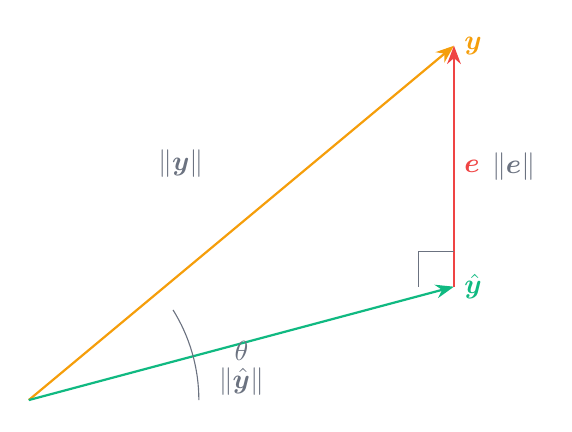
\begin{tikzpicture}[scale=1.8, >=Stealth]
  % Axes
  \draw[->, thick, response] (0,0) -- (3,2.5) node[right]{$\by$};
  \draw[->, thick, projection] (0,0) -- (3,0.8) node[right]{$\yhat$};
  \draw[->, thick, residual] (3,0.8) -- (3,2.5) node[midway,right]{$\be$};
  % Right angle
  \draw[secondary] (2.75,0.8) -- (2.75,1.05) -- (3,1.05);
  % Angle arc
  \draw[secondary] (1.2,0) arc[start angle=0,end angle=32,radius=1.2];
  \node[secondary] at (1.5,0.35) {$\theta$};
  % Labels
  \node[below,secondary] at (1.5,0.3) {$\norm{\yhat}$};
  \node[right,secondary] at (3.2,1.65) {$\norm{\be}$};
  \node[above left,secondary] at (1.3,1.5) {$\norm{\by}$};
\end{tikzpicture}
\caption{The regression right triangle. The Pythagorean theorem gives
$\text{SST}=\text{SSR}+\text{SSE}$.}
\end{figure}

\subsection{$R^2$ is the cosine of an angle}\label{sec:r2}

The coefficient of determination $R^2$ is usually introduced via the formula
$R^2 = 1 - \text{SSE}/\text{SST}$, or equivalently
$R^2 = \text{SSR}/\text{SST}$.
Let us derive this from the geometry of the regression right triangle.

Look at the right triangle in the figure above.
The \emph{hypotenuse} is the demeaned data vector $\tilde{\by}$ (with length $\sqrt{\text{SST}}$),
the \emph{adjacent side} is the demeaned fitted vector $\tilde{\yhat}$ (with length $\sqrt{\text{SSR}}$),
and the \emph{opposite side} is the residual $\be$ (with length $\sqrt{\text{SSE}}$).
The angle $\theta$ sits at the origin, between the hypotenuse and the adjacent side.

From basic trigonometry, the cosine of an angle in a right triangle is
\[
  \cos\theta = \frac{\text{adjacent}}{\text{hypotenuse}}
  = \frac{\norm{\tilde{\yhat}}}{\norm{\tilde{\by}}}
  = \frac{\sqrt{\text{SSR}}}{\sqrt{\text{SST}}}.
\]
Squaring both sides:
\[
  \cos^2\theta
  = \frac{\norm{\tilde{\yhat}}^2}{\norm{\tilde{\by}}^2}
  = \frac{\text{SSR}}{\text{SST}}.
\]
But $\text{SSR}/\text{SST}$ is precisely the definition of $R^2$, so we arrive at
\begin{equation}\label{eq:r2}
  \boxed{R^2 = \cos^2\theta = \frac{\text{SSR}}{\text{SST}}
  = 1 - \frac{\text{SSE}}{\text{SST}}.}
\end{equation}
The last equality follows directly from $\text{SST} = \text{SSR} + \text{SSE}$.

\begin{keyinsight}
$R^2$ is literally the squared cosine of the angle between the data vector
and its projection.
\begin{itemize}[nosep]
  \item When $\theta\approx 0$, the data vector nearly lies on the column space.
    The shadow almost coincides with the object, meaning the model explains
    nearly all the variability: $R^2\approx 1$.
  \item When $\theta\approx 90^\circ$, the data vector is nearly perpendicular to the
    column space.  The shadow is tiny---the model explains almost nothing:
    $R^2\approx 0$.
  \item $R^2 = 0.75$ means $\cos^2\theta = 0.75$, so $\theta\approx 30^\circ$.
    Three-quarters of the data's variability is captured by the
    projection; one quarter is residual.
\end{itemize}
\end{keyinsight}

% OP-4.2: INSERT Example 2 (Pythagoras Checks Out)
\begin{example}[Pythagoras Checks Out]\label{ex:pythagoras}
We continue with the data from Example~\ref{ex:first-regression}:
$\by = (1,3,2)^\top$, $\yhat = (3/2,\, 2,\, 5/2)^\top$,
$\be = (-1/2,\, 1,\, -1/2)^\top$.

The sample mean is $\bar{y} = (1+3+2)/3 = 2$, so the mean vector is
$\bar{y}\bm{1} = (2, 2, 2)^\top$.

\medskip\noindent\textbf{Step 1: Compute the three sums of squares.}

\emph{Total sum of squares} (deviation of $\by$ from its mean):
\[
\text{SST} = \norm{\by - \bar{y}\bm{1}}^2
= (1-2)^2 + (3-2)^2 + (2-2)^2
= 1 + 1 + 0 = 2.
\]
\emph{Regression sum of squares} (deviation of $\yhat$ from the mean):
\[
\text{SSR} = \norm{\yhat - \bar{y}\bm{1}}^2
= (3/2-2)^2 + (2-2)^2 + (5/2-2)^2
= 1/4 + 0 + 1/4 = 1/2.
\]
\emph{Residual sum of squares} (length of the residual):
\[
\text{SSE} = \norm{\be}^2
= (-1/2)^2 + 1^2 + (-1/2)^2
= 1/4 + 1 + 1/4 = 3/2.
\]

\medskip\noindent\textbf{Step 2: Verify Pythagoras.}
\[
\text{SSR} + \text{SSE} = \frac{1}{2} + \frac{3}{2} = 2 = \text{SST}.\;\checkmark
\]
This is the Pythagorean theorem in $\R^3$:
the squared hypotenuse $\norm{\by - \bar{y}\bm{1}}^2$ equals the sum of the two squared legs
$\norm{\yhat - \bar{y}\bm{1}}^2 + \norm{\be}^2$.
This works because $\yhat - \bar{y}\bm{1}$ and $\be$ are orthogonal---they live in perpendicular subspaces.

\medskip\noindent\textbf{Step 3: Compute $R^2$ as $\cos^2\theta$.}
\[
R^2 = \frac{\text{SSR}}{\text{SST}} = \frac{1/2}{2} = \frac{1}{4} = 0.25.
\]
Since $R^2 = \cos^2\theta$ where $\theta$ is the angle between
$\by - \bar{y}\bm{1}$ and $\yhat - \bar{y}\bm{1}$:
\[
\cos\theta = \sqrt{R^2} = \sqrt{1/4} = 1/2,
\qquad
\theta = \arccos(1/2) = 60^\circ.
\]

\medskip\noindent\textbf{Interpretation.}
The angle between the centered data vector and its shadow
is $60^\circ$---rather far from $0^\circ$ (perfect fit) and closer to $90^\circ$ (no fit at all).
The model explains only $25\%$ of the variance.
Geometrically, the shadow on the regression plane captures only
a quarter of the squared length of the centered data vector;
the remaining three-quarters is in the perpendicular residual direction.

\medskip\noindent\textbf{Takeaway.}
$R^2$ is literally the cosine-squared of the angle between the centered
observation vector and its projection.
A small angle means a long shadow and a good fit;
a large angle means the data point hovers far above the column space.
\end{example}

% OP-4.3: INSERT shadow-sharpness analogy
\medskip
\noindent\textbf{The shadow-sharpness analogy.}
Think of $R^2$ as measuring how \emph{sharp} a shadow is.
When the flashlight is nearly aligned with the data vector
($\theta \approx 0$), the shadow $\yhat$ is almost as long as the
object $\by$---the shadow is a crisp, faithful reproduction of the
object ($R^2 \approx 1$).

When the flashlight is nearly perpendicular to the data
($\theta \approx 90^\circ$), the shadow shrinks to almost nothing---a
tiny smudge that preserves none of the object's structure ($R^2 \approx 0$).

A shadow with $R^2 = 0.5$ (i.e.\ $\theta = 45^\circ$) preserves half
the object's ``energy'' (squared length).
The shadow exists, but it is a washed-out version of the original.
Whether that is good enough depends on what you need the shadow for.

% OP-4.4: INSERT Misconception 2 ("R^2 = 0.8 means good")
\begin{misconception}
\textbf{``$R^2 = 0.8$ means the model is good.''}

$R^2$ measures a geometric angle---nothing more.
A high $R^2$ does \emph{not} mean:
\begin{itemize}[nosep]
  \item The model is correctly specified (you might have the wrong
        functional form or omitted variables).
  \item The model will predict well out of sample (overfitting
        inflates $R^2$ on training data).
  \item The coefficients are meaningful (multicollinearity can give
        $R^2 = 0.99$ with wildly unstable individual coefficients).
\end{itemize}
Conversely, a low $R^2$ does \emph{not} mean the model is useless.
In fields with inherently noisy data (e.g.\ daily stock returns),
$R^2 = 0.03$ can represent an economically significant and
statistically reliable effect.

$R^2$ answers exactly one question: ``What fraction of the total
variability in $\by$ is captured by the projection onto $\Col(\bX)$?''
Whether that fraction is ``good enough'' depends on the scientific
context, not on any universal threshold.
\end{misconception}

% OP-4.5: INSERT Stop-and-Think 3 (adding noise columns)
\begin{stopandthink}
\textbf{Thought experiment: adding a random noise column.}

Suppose your current model has $R^2 = 0.60$.
You add a new column $\bm{z}$ to $\bX$, where $\bm{z}$ is pure random noise
(independent of everything).
\begin{enumerate}[nosep]
  \item Will SSE increase, decrease, or stay the same?
        \emph{Hint:} adding a column enlarges $\Col(\bX)$.
  \item Will SSR increase, decrease, or stay the same?
  \item Will $R^2$ increase, decrease, or stay the same?
  \item If you keep adding random noise columns until $p = n$,
        what happens to $R^2$?
\end{enumerate}
\emph{Answers:}
(1)~SSE can only decrease (or stay the same)---the projection onto a
larger subspace is always at least as close.
(2)~Since SST is fixed and SSE decreases, SSR must increase.
(3)~$R^2$ increases---even though the new column is pure noise!
(4)~When $p = n$, $\Col(\bX) = \R^n$, so $\yhat = \by$, $\be = \bm{0}$,
and $R^2 = 1$. The model ``explains'' everything but predicts nothing.
This is why $R^2$ alone is not a reliable measure of model quality.
\end{stopandthink}


\subsection{The Gauss--Markov theorem: OLS is the closest point}

% OP-4.6: REPLACE the Gauss-Markov proof sketch with full proof from round2_math
\begin{theorem}[Gauss--Markov]\label{thm:gm}
Assume $E[\bm{\varepsilon}] = \bm{0}$ and
$\text{Var}(\bm{\varepsilon}) = \sigma^2\bI_n$
(no assumption on the distribution of $\bm{\varepsilon}$).
Among all linear unbiased estimators of $\bm{c}^\top\bm{\beta}$
(for any fixed $\bm{c}\in\R^p$), the OLS estimator
$\bm{c}^\top\bhat = \bm{c}^\top(\bX^\top\bX)^{-1}\bX^\top\by$
has the smallest variance.
In the vector form: for any linear unbiased estimator
$\btilde = \bm{C}\by$ of $\bm{\beta}$,
\[
  \text{Var}(\btilde) - \text{Var}(\bhat) \;\succeq\; \bm{0}
  \qquad\text{(positive semi-definite).}
\]
\end{theorem}

\begin{proof}
\textbf{Step 1: Set up the alternative estimator.}
Let $\btilde = \bm{C}\by$ be any linear estimator of $\bm{\beta}$, where
$\bm{C}\in\R^{p\times n}$.  Write
\[
  \bm{C} = (\bX^\top\bX)^{-1}\bX^\top + \bD,
\]
where $\bD = \bm{C} - (\bX^\top\bX)^{-1}\bX^\top$ is the ``excess'' beyond
the OLS matrix.

\medskip
\noindent\textbf{Step 2: Derive the constraint from unbiasedness.}
For $\btilde$ to be unbiased for $\bm{\beta}$, we need
$E[\btilde] = \bm{\beta}$ for \emph{every} $\bm{\beta}\in\R^p$.
Since $\by = \bX\bm{\beta} + \bm{\varepsilon}$:
\begin{align*}
  E[\btilde]
  &= \bm{C}\,E[\by]
   = \bm{C}\bX\bm{\beta}
   = \bigl[(\bX^\top\bX)^{-1}\bX^\top + \bD\bigr]\bX\bm{\beta} \\
  &= \bI_p\bm{\beta} + \bD\bX\bm{\beta}
   = (\bI_p + \bD\bX)\bm{\beta}.
\end{align*}
For this to equal $\bm{\beta}$ for every $\bm{\beta}$, we need
\begin{equation}\label{eq:gm-constraint}
  \boxed{\bD\bX = \bm{0}.}
\end{equation}
This is the key constraint: the rows of $\bD$ must be orthogonal to the
columns of $\bX$.  In other words, $\bD$ maps the column space $\Col(\bX)$
to zero.

\medskip
\noindent\textbf{Step 3: Compute the variance and decompose.}
The variance of $\btilde$ is
\begin{align*}
  \text{Var}(\btilde)
  &= \bm{C}\,\text{Var}(\by)\,\bm{C}^\top
   = \sigma^2\bm{C}\bm{C}^\top \\
  &= \sigma^2\bigl[(\bX^\top\bX)^{-1}\bX^\top + \bD\bigr]
              \bigl[\bX(\bX^\top\bX)^{-1} + \bD^\top\bigr].
\end{align*}
Expanding the product:
\begin{align*}
  \bm{C}\bm{C}^\top
  &= (\bX^\top\bX)^{-1}\underbrace{\bX^\top\bX}_{}(\bX^\top\bX)^{-1}
     + (\bX^\top\bX)^{-1}\bX^\top\bD^\top
     + \bD\bX(\bX^\top\bX)^{-1}
     + \bD\bD^\top \\
  &= (\bX^\top\bX)^{-1}
     + (\bX^\top\bX)^{-1}\underbrace{(\bD\bX)^\top}_{\bm{0}}
     + \underbrace{\bD\bX}_{\bm{0}}(\bX^\top\bX)^{-1}
     + \bD\bD^\top,
\end{align*}
where the cross terms vanish by the constraint $\bD\bX = \bm{0}$.
Therefore:
\[
  \text{Var}(\btilde)
  = \sigma^2(\bX^\top\bX)^{-1} + \sigma^2\bD\bD^\top
  = \text{Var}(\bhat) + \sigma^2\bD\bD^\top.
\]

\medskip
\noindent\textbf{Step 4: Conclude.}
The matrix $\bD\bD^\top$ is positive semi-definite (for any vector $\bm{v}$,
$\bm{v}^\top\bD\bD^\top\bm{v} = \norm{\bD^\top\bm{v}}^2 \ge 0$).
Therefore
\[
  \boxed{
  \text{Var}(\btilde) - \text{Var}(\bhat)
  = \sigma^2\bD\bD^\top \succeq \bm{0}.
  }
\]
Equality holds if and only if $\bD = \bm{0}$, i.e., $\bm{C} = (\bX^\top\bX)^{-1}\bX^\top$.
The OLS estimator is the unique Best Linear Unbiased Estimator (BLUE).
\end{proof}

\begin{remark}[Geometric reading of Gauss--Markov]
The constraint $\bD\bX = \bm{0}$ says that the rows of $\bD$ live in
$\Col(\bX)^\perp$.  Any linear unbiased estimator that differs from OLS
must ``reach into'' the orthogonal complement of the column space to
form its estimate.  But $\Col(\bX)^\perp$ is exactly where the noise lives
(the residual space).  The extra term $\sigma^2\bD\bD^\top$ is the
variance penalty for picking up noise from outside the column space.
OLS is optimal precisely because it ignores everything orthogonal to
$\Col(\bX)$.
\end{remark}

\subsection{$R^2$ monotonicity}

\begin{proposition}\label{prop:r2mono}
Adding a predictor to $\bX$ can only increase (or maintain) $R^2$.
\end{proposition}

\begin{proof}
Adding a column to $\bX$ enlarges $\Col(\bX)$.
A projection onto a \emph{larger} subspace is at least as close to
$\by$ as a projection onto a smaller one, so $\norm{\be}^2$ cannot
increase, hence $R^2 = 1 - \norm{\be}^2/\text{SST}$ cannot decrease.
\end{proof}

\begin{warning}
$R^2$ monotonicity is a geometric fact about the \emph{training sample}.
It says nothing about out-of-sample prediction.
Adding polynomial terms ($x, x^2,\dots,x^{12}$) drives $R^2$ toward 1
while destroying predictive performance---the shadow gets closer in this
room but means nothing for the next room.
\end{warning}

% Breather: the Gauss-Markov proof was dense; reset the reader before moving on.
\medskip
\noindent\textit{We have now established that OLS is the best linear unbiased estimator.
The next two short subsections return to a lighter question: how do we
fairly measure how much variance the model explains?}

% OP-4.7: INSERT Adjusted R^2 subsection (geometric reading only)
\subsection{Adjusted $R^2$: paying for dimensions}\label{sec:adj-r2}

The monotonicity of $R^2$ (Proposition~\ref{prop:r2mono}) means that
$R^2$ can never decrease when we add predictors, even useless ones.
This makes raw $R^2$ unreliable for model comparison.
The \textbf{adjusted $R^2$} corrects for this by penalising model complexity.

\begin{definition}[Adjusted $R^2$]
\[
  R^2_{\text{adj}}
  = 1 - \frac{\text{SSE}/(n-p)}{\text{SST}/(n-1)}
  = 1 - \frac{n-1}{n-p}\,(1-R^2).
\]
\end{definition}

\noindent\textbf{Geometric reading.}
Think of the data vector $\by$ living in $\R^n$.
The column space $\Col(\bX)$ has dimension $p$, and the residual space
$\Col(\bX)^\perp$ has dimension $n - p$.
When we project $\by$ onto a $p$-dimensional subspace, we are ``using up''
$p$ dimensions to capture signal.  Even pure noise, projected onto a
$p$-dimensional subspace, produces a nonzero shadow---on average, the
squared length of this shadow is $p\sigma^2$.

The residual $\be$ lives in the remaining $n-p$ dimensions.
If the model captures no real signal, we expect
$\norm{\be}^2 \approx (n-p)\sigma^2$ (noise spread over $n-p$ dimensions)
and $\text{SST} \approx (n-1)\sigma^2$ (noise spread over $n-1$ dimensions,
after demeaning).
The ratio $\frac{\text{SSE}/(n-p)}{\text{SST}/(n-1)}$ then hovers around 1,
giving $R^2_{\text{adj}} \approx 0$---correctly indicating no explanatory power.

In short, $R^2_{\text{adj}}$ accounts for the fact that \emph{projecting onto
a subspace costs degrees of freedom}: each dimension consumed by the model
must ``earn its keep'' by reducing the residual more than random chance would.

% OP-4.8: INSERT Degrees of Freedom subsection (without d.f. bookkeeping remark)
\subsection{Degrees of freedom: the dimension of the residual space}\label{sec:df}

The phrase ``degrees of freedom'' appears throughout statistics, often without
geometric motivation.  The projection framework makes it transparent.

\begin{definition}[Degrees of freedom of the residual]
In a linear model with $p$ parameters fitted to $n$ observations, the
\textbf{residual degrees of freedom} is $n - p$.
\end{definition}

\noindent\textbf{Geometric interpretation.}
The data vector $\by$ lives in $\R^n$.
The projection $\yhat = \bH\by$ lives in $\Col(\bX)$, which has dimension $p$.
The residual $\be = \bM\by$ lives in $\Col(\bX)^\perp$, which has dimension
\[
  \dim\bigl(\Col(\bX)^\perp\bigr) = n - \dim\bigl(\Col(\bX)\bigr) = n - p.
\]
This is confirmed algebraically: $\rank(\bM) = \tr(\bM) = \tr(\bI_n - \bH) = n - p$.

The residual vector $\be\in\R^n$ has $n$ components, but it satisfies $p$
linear constraints ($\bX^\top\be = \bm{0}$, i.e., $\be\perp\Col(\bX)$).
So $\be$ is free to vary in only $n - p$ dimensions.
That is the number of ``degrees of freedom'' left after fitting the model.

\begin{remark}[Why divide by $n-p$, not $n$]
The unbiased estimator of $\sigma^2$ is
\[
  s^2 = \frac{\norm{\be}^2}{n - p} = \frac{\text{SSE}}{n-p},
\]
not $\norm{\be}^2/n$.  The geometric reason: $\be = \bM\bm{\varepsilon}$
(since $\bM\bX = \bm{0}$), and the expected squared length of
$\bm{\varepsilon}$ projected onto a $(n-p)$-dimensional subspace is
\[
  E[\norm{\bM\bm{\varepsilon}}^2]
  = E[\bm{\varepsilon}^\top\bM\bm{\varepsilon}]
  = \sigma^2\tr(\bM)
  = (n-p)\sigma^2.
\]
(Here we used $E[\bm{\varepsilon}\bm{\varepsilon}^\top] = \sigma^2\bI$
and the trace-expectation identity.)
Dividing by $n-p$ exactly compensates for the dimensionality of the
space into which the noise is projected, yielding $E[s^2] = \sigma^2$.

Dividing by $n$ would systematically underestimate $\sigma^2$, because
$p$ dimensions of the noise have been ``absorbed'' by the projection
onto $\Col(\bX)$---the hat matrix captures $p$ dimensions worth of noise
as spurious fit.
\end{remark}

% OP-4.9: INSERT transition sentence (Section 4 -> Section 5)
\medskip
\noindent\textit{So far, we have treated the column space as a monolithic
object and projected $\by$ onto it in one step.
But in multiple regression, different predictors contribute different
pieces of information.
Can we tease apart the contributions?
What does it really mean to ``control for'' a variable?
The Frisch--Waugh--Lovell theorem answers this by decomposing the
single projection into sequential steps.}


%======================================================================
\section{Peeling Apart the Variables: Frisch--Waugh--Lovell}\label{sec:fwl}
%======================================================================

\subsection{What ``controlling for'' means geometrically}

\noindent\textbf{What does ``conditioning on'' or ``controlling for'' a variable mean?}

In everyday regression language, you will hear phrases like
``the effect of education on income, \emph{controlling for} age'' or
``the coefficient of $x_2$ \emph{conditional on} $x_1$.''
For an undergraduate, this can sound mysterious.
Here is the plain-English idea:

Suppose you want to know whether education affects income.
But older people tend to have both more education and higher income simply because they have been working longer.
If you just regress income on education, you cannot tell whether the apparent effect comes from education itself or from age lurking in the background.
\emph{Controlling for age} means: compare people \emph{of the same age} and then ask whether more education is still associated with higher income.
In other words, you strip out the age-related variation from both income and education, and then look at what remains.

In a regression with multiple predictors, this is \emph{exactly} what the
coefficient of a predictor measures. When we write
$\by = \bX_1\bm{\beta}_1 + \bX_2\bm{\beta}_2 + \be$,
the coefficient $\bhat_2$ answers: \emph{what is the effect of $\bX_2$
after removing (``partialling out'') the influence of $\bX_1$?}
The Frisch--Waugh--Lovell theorem below makes this operation precise.

\begin{theorem}[Frisch--Waugh--Lovell]\label{thm:fwl}
Partition the design matrix as $\bX = [\bX_1\;\;\bX_2]$
with conformable coefficient vector $\bm{\beta}=(\bm{\beta}_1^\top,\bm{\beta}_2^\top)^\top$.
Let $\bM_1 = \bI - \bX_1(\bX_1^\top\bX_1)^{-1}\bX_1^\top$ be the
annihilator for $\Col(\bX_1)$.
Then
\begin{equation}\label{eq:fwl}
  \bhat_2 = (\bX_2^\top\bM_1\bX_2)^{-1}\bX_2^\top\bM_1\by.
\end{equation}
That is, $\bhat_2$ from the full regression equals the OLS coefficient
from regressing $\bM_1\by$ on $\bM_1\bX_2$---the
\emph{residualised} response on the \emph{residualised} predictors.
\end{theorem}

% OP-5.1: REPLACE the FWL proof with full block-elimination proof from round2_math
\begin{proof}
The normal equations $\bX^\top\bX\,\bhat = \bX^\top\by$ in block form are
\begin{equation}\label{eq:fwl-blocks}
  \begin{pmatrix}
    \bX_1^\top\bX_1 & \bX_1^\top\bX_2 \\
    \bX_2^\top\bX_1 & \bX_2^\top\bX_2
  \end{pmatrix}
  \begin{pmatrix}\bhat_1 \\ \bhat_2\end{pmatrix}
  =
  \begin{pmatrix}\bX_1^\top\by \\ \bX_2^\top\by\end{pmatrix}.
\end{equation}

\noindent\textbf{Step 1: Solve the first block for $\bhat_1$.}
The first block equation reads
\[
  \bX_1^\top\bX_1\,\bhat_1 + \bX_1^\top\bX_2\,\bhat_2
  = \bX_1^\top\by.
\]
Since $\bX_1$ has full column rank, $\bX_1^\top\bX_1$ is invertible, giving
\begin{equation}\label{eq:fwl-beta1}
  \bhat_1
  = (\bX_1^\top\bX_1)^{-1}\bX_1^\top\by
    - (\bX_1^\top\bX_1)^{-1}\bX_1^\top\bX_2\,\bhat_2.
\end{equation}

\noindent\textbf{Step 2: Substitute into the second block.}
The second block equation reads
\[
  \bX_2^\top\bX_1\,\bhat_1 + \bX_2^\top\bX_2\,\bhat_2
  = \bX_2^\top\by.
\]
Substituting~\eqref{eq:fwl-beta1}:
\begin{align*}
  \bX_2^\top\bX_1
  \bigl[(\bX_1^\top\bX_1)^{-1}\bX_1^\top\by
        &- (\bX_1^\top\bX_1)^{-1}\bX_1^\top\bX_2\,\bhat_2\bigr]
  + \bX_2^\top\bX_2\,\bhat_2
  = \bX_2^\top\by.
\end{align*}
Expanding and rearranging:
\begin{align*}
  &\bX_2^\top\underbrace{\bX_1(\bX_1^\top\bX_1)^{-1}\bX_1^\top}_{\bI - \bM_1}\by
  - \bX_2^\top\underbrace{\bX_1(\bX_1^\top\bX_1)^{-1}\bX_1^\top}_{\bI - \bM_1}\bX_2\,\bhat_2
  + \bX_2^\top\bX_2\,\bhat_2
  = \bX_2^\top\by.
\end{align*}
Since $\bX_1(\bX_1^\top\bX_1)^{-1}\bX_1^\top = \bI - \bM_1$, we can write:
\begin{align*}
  \bX_2^\top(\bI - \bM_1)\by
  &+ \bigl[\bX_2^\top\bX_2
     - \bX_2^\top(\bI - \bM_1)\bX_2\bigr]\bhat_2
  = \bX_2^\top\by.
\end{align*}

\noindent\textbf{Step 3: Simplify.}
Moving $\bX_2^\top(\bI-\bM_1)\by$ to the right-hand side:
\[
  \bX_2^\top\bM_1\bX_2\,\bhat_2
  = \bX_2^\top\by - \bX_2^\top(\bI-\bM_1)\by
  = \bX_2^\top\bM_1\by.
\]
Here we used $\bX_2^\top\bX_2 - \bX_2^\top(\bI-\bM_1)\bX_2 = \bX_2^\top\bM_1\bX_2$
and $\bX_2^\top\by - \bX_2^\top(\bI-\bM_1)\by = \bX_2^\top\bM_1\by$.

Since $\bM_1$ is symmetric and idempotent ($\bM_1^2 = \bM_1$, $\bM_1^\top = \bM_1$),
we have
\[
  \bX_2^\top\bM_1\bX_2 = \bX_2^\top\bM_1^\top\bM_1\bX_2
  = (\bM_1\bX_2)^\top(\bM_1\bX_2),
\]
which is the Gram matrix of the residualised predictors $\bM_1\bX_2$.
Similarly, $\bX_2^\top\bM_1\by = (\bM_1\bX_2)^\top(\bM_1\by)$.

Therefore, provided $\bM_1\bX_2$ has full column rank (i.e., $\bX_2$ is not
in $\Col(\bX_1)$),
\[
  \boxed{\bhat_2
  = \bigl[(\bM_1\bX_2)^\top(\bM_1\bX_2)\bigr]^{-1}(\bM_1\bX_2)^\top(\bM_1\by),}
\]
which is exactly the OLS estimator from regressing the residualised response
$\bM_1\by$ on the residualised predictors $\bM_1\bX_2$.
\end{proof}

\begin{keyinsight}
``Controlling for $\bX_1$'' is a geometric operation: project
$\by$ and $\bX_2$ onto the orthogonal complement of $\Col(\bX_1)$,
then perform simple regression in that cleaned-up space.
The multiple regression coefficient is the simple regression coefficient
in the residualised subspace.
\end{keyinsight}

\medskip
\noindent\textbf{The geometric analogy: two-step projection.}
Picture a three-dimensional room. The data vector $\by$ is a point floating in the room. The full column space $\Col(\bX_1, \bX_2)$ is a plane (the ``floor''). The subspace $\Col(\bX_1)$ is a line within that floor.

The FWL theorem says you can find the regression coefficient $\bhat_2$ via two sequential projections instead of one joint projection:
\begin{enumerate}[nosep]
  \item \textbf{Step 1: Remove $\bX_1$'s influence.}
    Project both $\by$ and $\bX_2$ onto the space \emph{perpendicular} to $\Col(\bX_1)$.
    This is like ``looking at the room from directly along the $\bX_1$ line''---the line collapses to a point, and only the variation perpendicular to $\bX_1$ remains visible.
    The residualised vectors $\bM_1\by$ and $\bM_1\bX_2$ live in this reduced space.
  \item \textbf{Step 2: Regress in the cleaned space.}
    Now perform a simple regression of $\bM_1\by$ on $\bM_1\bX_2$ in the reduced space.
    The resulting coefficient is exactly $\bhat_2$ from the full multiple regression.
\end{enumerate}
This two-step procedure is not an approximation---it gives the \emph{exact same} coefficient as the full regression.
Geometrically, the full projection onto the plane can be decomposed into a projection onto the line, followed by a projection of the remainder onto the perpendicular direction within the plane.

% OP-5.2: INSERT Example 3 (FWL by hand, corrected per round3_verification)
\begin{example}[FWL by Hand]\label{ex:fwl}
We have $n=4$ observations with two predictors:
\[
\begin{array}{c|ccc}
i & x_{1i} & x_{2i} & y_i \\\hline
1 & 1 & 0 & 2 \\
2 & 0 & 1 & 3 \\
3 & 1 & 1 & 6 \\
4 & 0 & 0 & 1
\end{array}
\]
Model: $y_i = \beta_0 + \beta_1 x_{1i} + \beta_2 x_{2i} + e_i$.
Notice that $x_1$ and $x_2$ have sample means $\bar{x}_1 = \bar{x}_2 = 1/2$
and sample covariance $-1/12$ (moderately negatively correlated among these four points).

\medskip\noindent\textbf{Part A: Full regression.}
\[
\bX = \begin{pmatrix}1&1&0\\1&0&1\\1&1&1\\1&0&0\end{pmatrix},\quad
\by=\begin{pmatrix}2\\3\\6\\1\end{pmatrix}.
\]
\[
\bX^\top\bX = \begin{pmatrix}4&2&2\\2&2&1\\2&1&2\end{pmatrix},\quad
\bX^\top\by = \begin{pmatrix}12\\8\\9\end{pmatrix}.
\]
Row reduction of the augmented matrix:
\[
\left(\begin{array}{ccc|c}
4&2&2&12\\2&2&1&8\\2&1&2&9
\end{array}\right)
\xrightarrow{R_2-\frac{1}{2}R_1,\;R_3-\frac{1}{2}R_1}
\left(\begin{array}{ccc|c}
4&2&2&12\\0&1&0&2\\0&0&1&3
\end{array}\right).
\]
Reading off: $\hat\beta_2 = 3$, $\hat\beta_1 = 2$,
$\hat\beta_0 = (12-2\cdot 2-2\cdot 3)/4 = (12-4-6)/4 = 1/2$.

So $\bhat = (1/2,\; 2,\; 3)^\top$, and in particular \fbox{$\hat\beta_2 = 3$}.

\emph{Verification:}
\[
\yhat = \begin{pmatrix}1/2+2+0\\1/2+0+3\\1/2+2+3\\1/2+0+0\end{pmatrix}
= \begin{pmatrix}5/2\\7/2\\11/2\\1/2\end{pmatrix},\quad
\be = \begin{pmatrix}2-5/2\\3-7/2\\6-11/2\\1-1/2\end{pmatrix}
= \begin{pmatrix}-1/2\\-1/2\\1/2\\1/2\end{pmatrix}.
\]
Check: $\bX^\top\be = (-1/2-1/2+1/2+1/2,\;-1/2+1/2,\;-1/2+1/2)^\top = (0,0,0)^\top$. $\checkmark$

\medskip\noindent\textbf{Part B: FWL two-step procedure for $\hat\beta_2$.}

Partition $\bX_1 = (\bm{1}\mid \bm{x}_1)$ (intercept and first predictor),
$\bX_2 = \bm{x}_2 = (0,1,1,0)^\top$.

\emph{Step B1: Compute $(\bX_1^\top\bX_1)^{-1}$.}
\[
\bX_1 = \begin{pmatrix}1&1\\1&0\\1&1\\1&0\end{pmatrix},\quad
\bX_1^\top\bX_1 = \begin{pmatrix}4&2\\2&2\end{pmatrix},\quad
\det=4,\quad
(\bX_1^\top\bX_1)^{-1} = \frac{1}{4}\begin{pmatrix}2&-2\\-2&4\end{pmatrix}
= \begin{pmatrix}1/2&-1/2\\-1/2&1\end{pmatrix}.
\]

\emph{Step B2: Residualise $\bm{x}_2$ on $\bX_1$.}

Regress $\bm{x}_2=(0,1,1,0)^\top$ on $\bX_1$:
\[
\bX_1^\top\bm{x}_2 = \begin{pmatrix}2\\1\end{pmatrix},\quad
(\bX_1^\top\bX_1)^{-1}\bX_1^\top\bm{x}_2
= \begin{pmatrix}1/2&-1/2\\-1/2&1\end{pmatrix}\begin{pmatrix}2\\1\end{pmatrix}
= \begin{pmatrix}1/2\\0\end{pmatrix}.
\]
Projection: $\bX_1\bigl(\begin{smallmatrix}1/2\\0\end{smallmatrix}\bigr)
= (1/2,\;1/2,\;1/2,\;1/2)^\top$.

Residual:
\[
\tilde{\bm{x}}_2 = (0,1,1,0)^\top - (1/2,1/2,1/2,1/2)^\top = (-1/2,\;1/2,\;1/2,\;-1/2)^\top.
\]
This is the part of $x_2$ not explained by the intercept and $x_1$---the ``new information'' that $x_2$ brings beyond what $x_1$ already provides.

% OP-12.1: CORRECTED Step B3 (arithmetic corrections from round3_verification)
\emph{Step B3: Residualise $\by$ on $\bX_1$.}
\[
\bX_1^\top\by = \begin{pmatrix}12\\8\end{pmatrix},\quad
(\bX_1^\top\bX_1)^{-1}\bX_1^\top\by
= \begin{pmatrix}1/2&-1/2\\-1/2&1\end{pmatrix}\begin{pmatrix}12\\8\end{pmatrix}
= \begin{pmatrix}2\\2\end{pmatrix}.
\]
Projection: $\bX_1\bigl(\begin{smallmatrix}2\\2\end{smallmatrix}\bigr)
= (2+2,\;2+0,\;2+2,\;2+0)^\top = (4,\;2,\;4,\;2)^\top$.

Residual:
\[
\tilde{\by} = (2,3,6,1)^\top - (4,2,4,2)^\top
= (-2,\;1,\;2,\;-1)^\top.
\]

\emph{Step B4: Regress $\tilde{\by}$ on $\tilde{\bm{x}}_2$ (no intercept needed---both have been purged of $\bX_1$).}
\[
\hat\beta_2^{\text{FWL}} = \frac{\tilde{\bm{x}}_2^\top\tilde{\by}}{\tilde{\bm{x}}_2^\top\tilde{\bm{x}}_2}.
\]
Numerator:
\[
\tilde{\bm{x}}_2^\top\tilde{\by}
= \bigl(-\tfrac{1}{2}\bigr)(-2) + \bigl(\tfrac{1}{2}\bigr)(1)
  + \bigl(\tfrac{1}{2}\bigr)(2) + \bigl(-\tfrac{1}{2}\bigr)(-1)
= 1 + \tfrac{1}{2} + 1 + \tfrac{1}{2} = 3.
\]
Denominator:
\[
\tilde{\bm{x}}_2^\top\tilde{\bm{x}}_2
= \tfrac{1}{4}+\tfrac{1}{4}+\tfrac{1}{4}+\tfrac{1}{4} = 1.
\]
Therefore:
\[
\boxed{\hat\beta_2^{\text{FWL}} = \frac{3}{1} = 3 = \hat\beta_2^{\text{full}}.}\;\checkmark
\]

\medskip\noindent\textbf{What happened geometrically?}
The FWL theorem says: to find the coefficient of $x_2$ in the full model,
first remove from both $\by$ and $\bm{x}_2$ everything that $\bX_1$ can explain.
Regressing the residual components on each other gives \emph{exactly}
the same coefficient as the full regression.

\medskip\noindent\textbf{Takeaway.}
FWL is not an approximation. The two-step residualisation procedure
recovers $\hat\beta_2 = 3$ exactly, because projection onto a direct sum
decomposes into sequential projections onto complementary subspaces.
\end{example}

% OP-5.3: INSERT Figure 3 (FWL two-step projection)
\begin{figure}[ht]
\centering
\tdplotsetmaincoords{62}{130}
\begin{tikzpicture}[tdplot_main_coords, scale=1.35, >=Stealth]

  % --- Full plane Col(X1,X2) ---
  \fill[colspace!8] (-3.2,-2.6,0) -- (3.2,-2.6,0) -- (3.2,2.6,0) -- (-3.2,2.6,0) -- cycle;
  \draw[colspace!30, line width=0.4pt]
    (-3.2,-2.6,0) -- (3.2,-2.6,0) -- (3.2,2.6,0) -- (-3.2,2.6,0) -- cycle;
  \node[colspace!70!black, font=\scriptsize\itshape] at (2.8,-2.1,0)
    {$\operatorname{Col}(\bm{X}_1,\bm{X}_2)$};

  % --- Col(X1) as a line in the plane ---
  \draw[colspace!70, very thick] (-2.8,-0.7,0) -- (2.8,0.7,0);
  \node[colspace!80!black, font=\scriptsize\itshape] at (2.9,1.0,0)
    {$\operatorname{Col}(\bm{X}_1)$};

  % --- x2 in the plane ---
  \draw[->, colspace!60!black, thick] (0,0,0) -- (1.0,2.2,0)
    node[above left, font=\scriptsize\bfseries] {$\bm{x}_2$};

  % --- y above the plane ---
  \coordinate (y) at (1.6,1.6,2.6);
  \draw[->, response, very thick] (0,0,0) -- (y)
    node[above right, font=\footnotesize\bfseries] {$\bm{y}$};

  % --- Projection of x2 onto Col(X1) ---
  \coordinate (px2) at (1.2,0.3,0);
  \draw[->, secondary, thin] (0,0,0) -- (px2);

  % --- M1 x2 = residualised x2 (in plane, perp to Col(X1)) ---
  \coordinate (m1x2) at (-0.2,1.9,0);
  \draw[->, constraint, thick] (px2) -- (1.0,2.2,0)
    node[midway, above left=-1pt, font=\scriptsize\bfseries] {$\bm{M}_1\bm{x}_2$};

  % --- Projection of y onto Col(X1): P1 y ---
  \coordinate (p1y) at (1.8,0.45,0);
  % --- M1 y: y residualised from Col(X1) ---
  \coordinate (m1y) at (-0.2,1.15,2.6);
  % Show M1 y from p1y direction... approximate as from y minus its Col(X1) component
  % For visual clarity: show M1y as a vector in the "orthogonal complement + z" direction
  \coordinate (m1yend) at (0.4,1.9,2.2);
  \draw[->, constraint!70!black, thick, dashed] (0,0,0) -- (m1yend)
    node[left=2pt, font=\scriptsize\bfseries] {$\bm{M}_1\bm{y}$};

  % --- Full projection yhat on the plane ---
  \coordinate (yhat) at (1.6,1.6,0);
  \draw[->, projection, very thick] (0,0,0) -- (yhat)
    node[below right=1pt, font=\footnotesize\bfseries] {$\hat{\bm{y}}$};

  % --- Residual e ---
  \draw[->, residual, thick, dashed] (yhat) -- (y)
    node[midway, right=2pt, font=\footnotesize\bfseries] {$\bm{e}$};

  % --- Step labels ---
  \node[constraint!80!black, font=\scriptsize, align=center,
    fill=white, fill opacity=0.85, text opacity=1, inner sep=2pt,
    rounded corners=1pt]
    at (-2.4,2.0,1.8)
    {\textbf{Step 1}\\[1pt]Residualise:\\$\bm{M}_1\bm{y}$, $\bm{M}_1\bm{x}_2$};

  \node[projection!80!black, font=\scriptsize, align=center,
    fill=white, fill opacity=0.85, text opacity=1, inner sep=2pt,
    rounded corners=1pt]
    at (3.0,1.8,1.4)
    {\textbf{Step 2}\\[1pt]Regress $\bm{M}_1\bm{y}$\\on $\bm{M}_1\bm{x}_2$};

  % --- Right angle at yhat ---
  \draw[secondary, line width=0.5pt]
    ($(yhat)+(-0.15,0,0)$) -- ($(yhat)+(-0.15,0,0.15)$) -- ($(yhat)+(0,0,0.15)$);

  % Origin
  \fill[secondary] (0,0,0) circle (1.2pt);
  \node[below left, secondary, font=\scriptsize] at (-0.1,-0.1,0) {$\bm{0}$};

\end{tikzpicture}
\caption{The Frisch--Waugh--Lovell theorem as a two-step projection.
\textbf{Step~1}: residualise both~$\bm{y}$ and~$\bm{x}_2$ with respect
to~$\operatorname{Col}(\bm{X}_1)$ using the annihilator~$\bm{M}_1$,
sweeping out the effect of~$\bm{X}_1$.
\textbf{Step~2}: regress~$\bm{M}_1\bm{y}$ on~$\bm{M}_1\bm{x}_2$ in the
reduced orthogonal complement.  The resulting coefficient~$\hat\beta_2$
is identical to the one obtained from the full regression, and the
final fitted vector~$\hat{\bm{y}}$ is the same.}
\label{fig:fwl}
\end{figure}

% OP-5.4: INSERT Stop-and-Think 4 (FWL limiting cases)
\begin{stopandthink}
\textbf{Two limiting cases of FWL.}

Recall that $\bhat_2 = (\bX_2^\top \bM_1 \bX_2)^{-1}\bX_2^\top \bM_1 \by$,
where $\bM_1 = \bI - \bH_1$ removes the influence of $\bX_1$.
\begin{enumerate}[nosep]
  \item \textbf{Case 1:} $\bX_1 \perp \bX_2$
    (i.e.\ $\bX_1^\top \bX_2 = \bm{0}$).
    What does $\bM_1 \bX_2$ simplify to?
    What does this tell you about the FWL coefficient $\bhat_2$
    compared to the coefficient from a simple regression of $\by$ on $\bX_2$ alone?
  \item \textbf{Case 2:} $\bX_2 \in \Col(\bX_1)$
    (i.e.\ $\bX_2$ is a linear combination of the columns of $\bX_1$).
    What does $\bM_1 \bX_2$ simplify to?
    What goes wrong?
\end{enumerate}
\emph{Answers:}
(1)~When $\bX_1 \perp \bX_2$, we have $\bH_1 \bX_2 = \bm{0}$, so
$\bM_1 \bX_2 = \bX_2$. The residualised predictor equals the original
predictor---controlling for $\bX_1$ changes nothing.
The FWL coefficient equals the simple regression coefficient.
This is why uncorrelated predictors give the same coefficients whether
you include them together or separately.

(2)~When $\bX_2 \in \Col(\bX_1)$, we have $\bH_1 \bX_2 = \bX_2$, so
$\bM_1 \bX_2 = \bm{0}$. The residualised predictor is the zero vector.
The formula $(\bX_2^\top \bM_1 \bX_2)^{-1}$ requires inverting a zero matrix,
which is impossible.
This is perfect multicollinearity: $\bX_2$ contains no information
beyond what $\bX_1$ already provides.
\end{stopandthink}

\subsection{The effect of predictor correlation}

The FWL theorem reveals \emph{why} correlated predictors cause trouble.
To understand this, think carefully about what the residualisation step does.

\medskip
\noindent\textbf{The residualised predictor and its length.}
When we ``control for'' $\bX_1$, we replace $\bX_2$ by its residuals after regressing on $\bX_1$:
\[
  \bM_1\bX_2 = \bX_2 - \underbrace{\bX_1(\bX_1^\top\bX_1)^{-1}\bX_1^\top\bX_2}_{\text{part of }\bX_2\text{ explained by }\bX_1}.
\]
The residualised predictor $\bM_1\bX_2$ contains only the ``unique information'' in $\bX_2$---the part that $\bX_1$ cannot account for.

Now think about what happens as the correlation between $\bX_1$ and $\bX_2$ changes:
\begin{itemize}[nosep]
  \item \textbf{Uncorrelated predictors} ($\bX_1^\top\bX_2 \approx \bm{0}$):
    The projection of $\bX_2$ onto $\Col(\bX_1)$ is nearly zero, so $\bM_1\bX_2 \approx \bX_2$.
    Almost all of $\bX_2$'s information is unique. The residualised predictor is long, and the coefficient is estimated precisely.
  \item \textbf{Moderately correlated predictors}:
    Part of $\bX_2$ is ``used up'' by $\bX_1$. The residualised predictor $\bM_1\bX_2$ is shorter. Less unique information remains, and the coefficient estimate becomes noisier.
  \item \textbf{Highly correlated predictors} ($\bX_2\approx \bX_1\bm{c}$ for some $\bm{c}$):
    Nearly all of $\bX_2$ is explained by $\bX_1$. The residualised predictor $\bM_1\bX_2$ is very short---close to the zero vector. There is almost no unique information left. The coefficient estimate becomes wildly unstable.
\end{itemize}

\medskip
\noindent\textbf{Geometric picture.}
Imagine $\bX_1$ and $\bX_2$ as two vectors in $\R^n$.
Residualising $\bX_2$ with respect to $\bX_1$ means projecting $\bX_2$ onto the plane perpendicular to $\bX_1$ and keeping only the perpendicular component.
If $\bX_2$ points in nearly the same direction as $\bX_1$, this perpendicular component is tiny.
You are trying to estimate a coefficient by regressing on a near-zero vector, which amplifies any noise enormously.

\medskip
\noindent\textbf{The standard error formula.}
The standard error of $\bhat_2$ is
\[
  \text{SE}(\hat{\beta}_{2,j})
  = \sqrt{\frac{s^2}{\norm{\bM_1\bm{x}_{2,j}}^2}},
\]
where $s^2 = \norm{\be}^2/(n-p)$ is the estimated residual variance.
As correlation increases, $\norm{\bM_1\bm{x}_{2,j}}\to 0$ and the denominator vanishes,
sending $\text{SE}\to\infty$.
This is the geometric root of \emph{multicollinearity}: the coefficient is not wrong on average (it is still unbiased), but it is estimated so imprecisely that it becomes practically useless.

% OP-5.5: INSERT transition sentence (Section 5 -> Section 6)
\medskip
\noindent\textit{FWL revealed that individual coefficients depend on
the unique information each predictor contributes, as measured by
the residualised predictor's length.
But some observations contribute more to the projection than others.
Which observations have the most influence on the fitted values,
and how can we detect problematic data points?}



%======================================================================
\section{Leverage and Influence}\label{sec:leverage}
%======================================================================

\subsection{Leverage as geometric distance}

Each fitted value $\hat{y}_i = \sum_j h_{ij}y_j$ is a weighted
combination of all responses. The diagonal element $h_{ii}$
measures how much observation $i$ influences \emph{its own} prediction.

\begin{definition}
The \textbf{leverage} of observation $i$ is $h_{ii}$, the $i$-th diagonal
element of $\bH$. By Proposition~\ref{prop:hat}(iv),
$0 \le h_{ii} \le 1$ and $\sum_i h_{ii} = p$.
The conventional threshold for ``high leverage'' is $h_{ii} > 2p/n$.
\end{definition}

\begin{remark}[The bound $h_{ii}\ge 1/n$ when an intercept is present]\label{rem:hii-intercept}
When the model includes an intercept (i.e., a column of ones $\bm{1}\in\Col(\bX)$),
the leverage satisfies the stronger bound $h_{ii}\ge 1/n$.
To see why: the hat matrix projects onto $\Col(\bX)$, which contains $\bm{1}$.
In particular, $\bH\bm{1} = \bm{1}$, so the $i$-th row of $\bH$ sums to 1:
$\sum_{j=1}^n h_{ij} = 1$.
This can be proved using the Cauchy--Schwarz inequality applied to the
rows of~$\bH$; the proof is in Appendix~\ref{app:proofs}.

Without an intercept, it is possible to have $h_{ii} = 0$ (for an observation
$\bm{x}_i$ orthogonal to every column of $\bX$), so the general bound is
$0 \le h_{ii} \le 1$.
\end{remark}

Geometrically, $h_{ii}$ measures how far the $i$-th predictor vector
$\bm{x}_i^\top$ lies from the centroid of the predictor space.
Observations in unusual predictor combinations have long ``arms''
in the tug-of-war that determines the projection.

\subsection{Cook's distance: leverage $\times$ surprise}

High leverage means an observation \emph{can} distort the projection.
Whether it \emph{does} depends on whether it also has a large residual.
Cook's distance combines both pieces of information into a single measure of \emph{influence}.

\medskip
\noindent\textbf{The thought experiment behind Cook's distance.}
Imagine deleting observation $i$ from the dataset and re-running the entire regression.
How much do the fitted values change?
If they barely move, observation $i$ is not influential.
If they change dramatically, observation $i$ is pulling the regression toward itself.

Cook's distance measures exactly this: it is proportional to the squared distance between the fitted values from the full regression and the fitted values with observation $i$ removed:
\[
  D_i \;\propto\; \norm{\yhat - \yhat_{(i)}}^2,
\]
where $\yhat_{(i)}$ denotes the fitted values from the regression that excludes observation $i$.
The remarkable fact is that you do not actually need to refit the regression $n$ times.
Using the hat matrix, Cook's distance can be computed in closed form.

\begin{definition}
\textbf{Cook's distance} for observation $i$ is
\[
  D_i = \frac{e_i^2}{p\cdot\text{MSE}}
        \cdot \frac{h_{ii}}{(1 - h_{ii})^2},
\]
where $\text{MSE} = \norm{\be}^2/(n-p)$ is the mean squared error.
\end{definition}

\noindent\textbf{Reading the formula.}
Cook's distance is a product of two factors:
\begin{enumerate}[nosep]
  \item $\frac{e_i^2}{p\cdot\text{MSE}}$ --- this is the \textbf{surprise factor}.
    It measures how large the residual of observation $i$ is, relative to the overall noise level.
    A large residual means the observation does not fit the current model well; it ``wants'' the regression plane to tilt toward it.
  \item $\frac{h_{ii}}{(1 - h_{ii})^2}$ --- this is the \textbf{leverage factor}.
    It measures how much ``mechanical advantage'' the observation has.
    An observation at an extreme predictor value ($h_{ii}$ close to 1) can exert enormous force on the regression; an observation near the center of the predictor cloud ($h_{ii}$ close to $1/n$) has little leverage, no matter how unusual its $y$-value.
\end{enumerate}

\medskip
\noindent\textbf{An analogy.}
Think of the regression line as a seesaw (lever) balanced on the centroid of the data.
\emph{Leverage} ($h_{ii}$) is how far from the fulcrum observation $i$ sits---its position along the seesaw.
The \emph{residual} ($e_i$) is the force it pushes with---how far above or below the seesaw it is.
Cook's distance is the resulting \emph{torque}: force times distance from the fulcrum.
A person sitting at the end of the seesaw (high leverage) and pushing hard (large residual) tilts the seesaw a lot. A person sitting near the fulcrum (low leverage), no matter how hard they push, barely tilts it.

\medskip
\noindent\textbf{When to worry.}
A common rule of thumb is to investigate observations with $D_i > 4/n$ or $D_i > 1$.
But the real message is qualitative: look at observations with large Cook's distance
and ask whether they represent data errors, unusual subpopulations, or genuine outliers
that should influence the model.

\begin{keyinsight}
\textbf{Influence = leverage $\times$ surprise.}
An observation needs \emph{both} a long arm ($h_{ii}$ large) \emph{and}
a strong pull ($|e_i|$ large) to actually move the regression.
A high-leverage observation that fits the trend is harmless
(large $h_{ii}$, small $e_i$, so $D_i$ is small).
A central observation with a large residual has limited impact
(small $h_{ii}$, large $e_i$, so $D_i$ is moderate).
The dangerous case is an observation that is \emph{both} extreme in its
predictor values \emph{and} does not follow the pattern of the other data.
\end{keyinsight}


%======================================================================
\section{When the Geometry Fails}\label{sec:failures}
%======================================================================

\subsection{Multicollinearity: the geometry breaks}\label{sec:multicollinearity}

When predictors are nearly linearly dependent, $\Col(\bX)$ degenerates
from a ``thick'' plane into a paper-thin sliver.
Let us understand why this is dangerous and what exactly goes wrong.

\medskip
\noindent\textbf{What multicollinearity means.}
Multicollinearity occurs when one predictor can be approximately written as a linear combination of others.
For example, if $x_2 \approx 3x_1 + 2x_3$, then the three predictors contain nearly the same information.
The design matrix $\bX$ is close to being rank-deficient.

\medskip
\begin{remark}[Prerequisite: eigendecomposition of symmetric matrices]
Before proceeding, let us recall a fundamental fact from linear algebra.

Every real symmetric matrix $\bm{A} \in \R^{p \times p}$ can be
decomposed as
\[
  \bm{A} = \bQ \bm{\Lambda} \bQ^\top,
\]
where $\bQ = [\bm{q}_1 \mid \cdots \mid \bm{q}_p]$ is an orthogonal
matrix ($\bQ^\top \bQ = \bI$) whose columns are the \emph{eigenvectors},
and $\bm{\Lambda} = \diag(\lambda_1, \dots, \lambda_p)$ contains the
corresponding \emph{eigenvalues}.

Key properties:
\begin{itemize}[nosep]
  \item All eigenvalues of a real symmetric matrix are \emph{real}
        (not complex).
  \item The eigenvectors can be chosen to be \emph{orthonormal}.
  \item If $\bm{A}$ is also positive semi-definite (like $\bX^\top\bX$),
        all eigenvalues are non-negative: $\lambda_k \ge 0$.
  \item The eigenvalues measure the ``stretch'' of the matrix in each
        eigenvector direction: $\bm{A}\bm{q}_k = \lambda_k \bm{q}_k$.
\end{itemize}

The inverse (when it exists) is simply
$\bm{A}^{-1} = \bQ \bm{\Lambda}^{-1} \bQ^\top
= \bQ \, \diag(1/\lambda_1, \dots, 1/\lambda_p) \, \bQ^\top$.
This makes it clear that small eigenvalues produce large entries in the
inverse---the source of variance inflation under multicollinearity.
\end{remark}

\medskip
\noindent\textbf{Why it is dangerous: the pancake analogy.}
Consider fitting a model with two highly correlated predictors.
Geometrically, the column space $\Col(\bX)$ is a 2-dimensional plane in $\R^n$.
When the two predictors are nearly proportional, this plane is not a ``square'' plane---it is extremely elongated, like a thin pancake or a nearly 1-dimensional line.

Now imagine projecting the data vector $\by$ onto this thin pancake.
The projection itself is fine: $\yhat$ lands on the pancake and $\be$ is perpendicular.
The \emph{total} prediction $\yhat$ is stable.
But the \emph{individual coefficients} are not: there are many different ways to decompose $\yhat$ into contributions along two nearly parallel directions.
A tiny change in $\by$ can slide $\yhat$ along the pancake, dramatically changing the decomposition $(\hat{\beta}_1, \hat{\beta}_2)$ even though $\yhat = \hat{\beta}_1\bm{x}_1 + \hat{\beta}_2\bm{x}_2$ stays almost the same.

\medskip
\noindent\textbf{The eigenvalue perspective.}
The eigenvalue decomposition of $\bX^\top\bX$ makes this precise:
\[
  \bX^\top\bX = \bQ\bm{\Lambda}\bQ^\top,
  \qquad
  \bm{\Lambda} = \diag(\lambda_1,\dots,\lambda_p),
  \quad \lambda_1\ge\cdots\ge\lambda_p\ge 0.
\]
The eigenvalues measure the ``width'' of the column space in each principal direction.
A large eigenvalue $\lambda_k$ means the column space extends far in direction $\bm{q}_k$---the projection is stable there.
A small eigenvalue $\lambda_k$ means the column space is paper-thin in that direction---the projection's location is poorly determined.

The variance of the OLS coefficients is $\text{Var}(\bhat) = \sigma^2(\bX^\top\bX)^{-1} = \sigma^2\bQ\bm{\Lambda}^{-1}\bQ^\top$.
In the direction of the smallest eigenvalue, the variance is $\sigma^2/\lambda_p$---which explodes when $\lambda_p$ is small.

The \textbf{condition number} $\kappa = \lambda_1/\lambda_p$
measures the aspect ratio of the eigenvalue ellipsoid.
When $\kappa \gg 1$, the column space is elongated: the projection
onto the column space is stable (overall $R^2$ is fine), but the
projection's \emph{location within} the thin direction is wildly
unstable. Small perturbations in $\by$ cause large swings
in individual coefficients.

Figure~\ref{fig:multicollinearity} illustrates this contrast visually.

% --- Figure 4: Multicollinearity (placed within Section 7.1, after eigenvalue perspective) ---

\begin{figure}[ht]
\centering
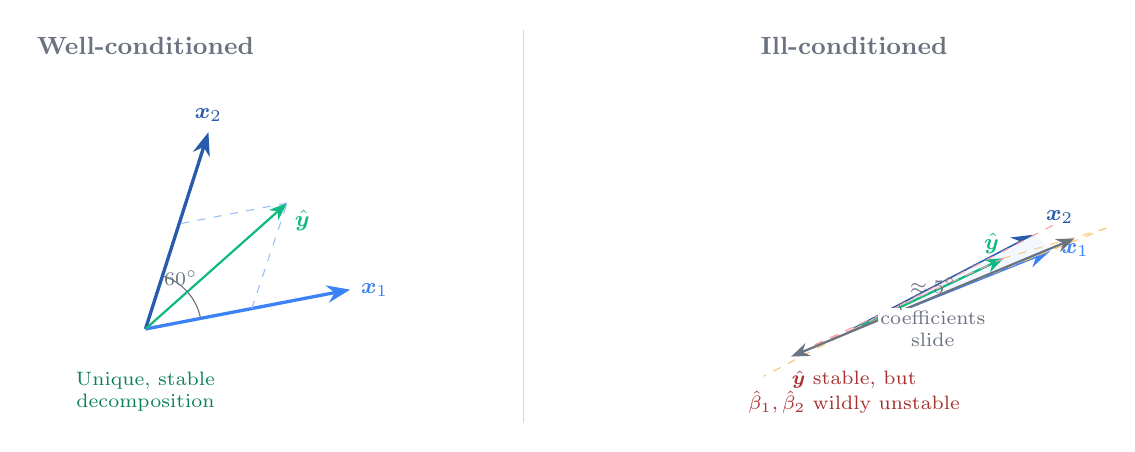
\begin{tikzpicture}[>=Stealth, scale=1.0]

  % ============== LEFT: Well-conditioned ==============
  \begin{scope}[shift={(-4.8,0)}]
    \node[secondary, font=\small\bfseries] at (0,3.6) {Well-conditioned};

    % Column vectors at ~60 degrees
    \draw[->, colspace, very thick] (0,0) -- (2.6,0.5)
      node[right, font=\footnotesize\bfseries] {$\bm{x}_1$};
    \draw[->, colspace!70!black, very thick] (0,0) -- (0.8,2.5)
      node[above, font=\footnotesize\bfseries] {$\bm{x}_2$};

    % Projection yhat
    \coordinate (yhat) at (1.8,1.6);
    \draw[->, projection, thick] (0,0) -- (yhat)
      node[below right=-1pt, font=\footnotesize\bfseries] {$\hat{\bm{y}}$};

    % Decomposition parallelogram
    \coordinate (comp1end) at (1.35,0.26);
    \draw[colspace!50, thin, dashed] (comp1end) -- (yhat);
    \draw[colspace!50, thin, dashed] (0.45,1.34) -- (yhat);

    % Angle arc
    \draw[secondary, thin] (0.7,0.135) arc[start angle=11,end angle=72,radius=0.71];
    \node[secondary, font=\scriptsize] at (0.45,0.65) {$60^\circ$};

    % Stable label
    \node[projection!70!black, font=\scriptsize, align=center] at (0,-0.8)
      {Unique, stable\\decomposition};
  \end{scope}

  % ============== RIGHT: Ill-conditioned ==============
  \begin{scope}[shift={(4.2,0)}]
    \node[secondary, font=\small\bfseries] at (0,3.6) {Ill-conditioned};

    % Column vectors nearly parallel
    \draw[->, colspace, very thick] (0,0) -- (2.5,1.0)
      node[right, font=\footnotesize\bfseries] {$\bm{x}_1$};
    \draw[->, colspace!70!black, very thick] (0,0) -- (2.3,1.2)
      node[above right, font=\footnotesize\bfseries] {$\bm{x}_2$};

    % Thin sliver region
    \fill[colspace!6] (0,0) -- (2.5,1.0) -- (2.3,1.2) -- cycle;

    % Projection yhat (stable)
    \coordinate (yhat) at (1.9,0.9);
    \draw[->, projection, thick] (0,0) -- (yhat)
      node[above left=-2pt, font=\footnotesize\bfseries] {$\hat{\bm{y}}$};

    % Decomposition 1
    \draw[response!60, thin, dashed] (0,0) -- (3.2,1.28);
    \draw[response!60, thin, dashed] (0,0) -- (-1.15,-0.6);
    \coordinate (d1a) at (3.2,1.28);
    \draw[response!50, thin, dashed] (d1a) -- (yhat);

    % Decomposition 2
    \draw[residual!50, thin, dashed] (0,0) -- (-0.5,-0.2);
    \draw[residual!50, thin, dashed] (0,0) -- (2.53,1.32);
    \coordinate (d2a) at (-0.5,-0.2);
    \draw[residual!50, thin, dashed] (d2a) -- (yhat);

    % Sliding annotation
    \draw[<->, secondary, thick] (2.8,1.15) -- (-0.8,-0.35);
    \node[secondary, font=\scriptsize, align=center, fill=white,
      inner sep=1pt] at (1.0,0.0)
      {coefficients\\slide};

    % Angle arc (small)
    \draw[secondary, thin] (0.6,0.24) arc[start angle=22,end angle=28,radius=0.64];
    \node[secondary, font=\scriptsize] at (1.0,0.55) {$\approx 5^\circ$};

    % Unstable label
    \node[residual!70!black, font=\scriptsize, align=center] at (0,-0.8)
      {$\hat{\bm{y}}$ stable, but\\$\hat\beta_1,\hat\beta_2$ wildly unstable};
  \end{scope}

  % Dividing line
  \draw[secondary!30, thin] (0,-1.2) -- (0,3.8);

\end{tikzpicture}
\caption{Multicollinearity as geometry.
\textbf{Left}: well-separated predictors give a stable decomposition.
\textbf{Right}: nearly collinear predictors create a thin sliver; the
projection~$\hat{\bm{y}}$ is stable but the individual coefficients
slide dramatically along the sliver direction.}
\label{fig:multicollinearity}
\end{figure}

\medskip
\noindent\textbf{The key danger, summarised.}
Multicollinearity does \emph{not} make the overall model bad---$R^2$ and the predicted values $\yhat$ may be perfectly fine.
What it destroys is the interpretability of individual coefficients.
You cannot say ``a one-unit increase in $x_2$ leads to a $\hat{\beta}_2$ change in $y$, holding $x_1$ constant'' when $x_1$ and $x_2$ move together so tightly that ``holding $x_1$ constant'' is practically impossible.

\medskip
\noindent\textbf{Diagnostic:} The condition number $\kappa$ and the
eigenvalue spectrum. If $\kappa > 30$, investigate; if $\kappa > 100$,
individual coefficients may be unreliable.
Another common diagnostic is the \textbf{Variance Inflation Factor}
(VIF): $\text{VIF}_j = 1/(1-R_j^2)$, where $R_j^2$ is the $R^2$ from
regressing predictor $x_j$ on all other predictors.
$\text{VIF}_j > 10$ is often flagged as concerning.

\begin{misconception}
\textbf{``Multicollinearity makes the model bad.''}

Multicollinearity inflates standard errors of individual coefficients,
but it does \emph{not}:
\begin{itemize}[nosep]
  \item Bias the OLS estimates (they remain unbiased).
  \item Ruin the overall prediction ($\yhat$ and $R^2$ can be fine).
  \item Invalidate the $F$-test for the joint significance of a group
        of collinear predictors.
\end{itemize}
Multicollinearity is only a problem \emph{if you need to interpret
individual coefficients}.
If your goal is prediction, collinear predictors may cause no harm
at all---the instability in individual $\hat{\beta}_j$ averages out in
$\yhat = \bX\bhat$.
\end{misconception}

\subsection{Omitted variable bias: the geometry can't warn you}

\begin{warning}
Multicollinearity is a problem the geometry can \emph{see}.
Omitted variable bias is a problem the geometry \emph{cannot} see.
\end{warning}

Suppose the true model is
$\by = \bX_1\bm{\beta}_1 + \bX_2\bm{\beta}_2 + \bm{\varepsilon}$
but we estimate the ``short'' regression omitting $\bX_2$:
\[
  \bhat_1^{\text{short}}
  = (\bX_1^\top\bX_1)^{-1}\bX_1^\top\by
  = \bm{\beta}_1 + \underbrace{(\bX_1^\top\bX_1)^{-1}\bX_1^\top\bX_2}_{\bm{\Gamma}}\bm{\beta}_2
    + (\bX_1^\top\bX_1)^{-1}\bX_1^\top\bm{\varepsilon}.
\]
Taking expectations:
\begin{equation}\label{eq:ovb}
  \boxed{
  E[\bhat_1^{\text{short}}] = \bm{\beta}_1 + \bm{\Gamma}\bm{\beta}_2.
  }
\end{equation}
The bias $\bm{\Gamma}\bm{\beta}_2$ is the gap between projections onto
two different column spaces.
It exists whenever (i) $\bX_2$ is correlated with $\bX_1$
($\bm{\Gamma}\ne\bm{0}$) \emph{and} (ii) $\bX_2$ affects $\by$
($\bm{\beta}_2\ne\bm{0}$).

Both the short and long regressions have perfectly orthogonal residuals,
healthy condition numbers, and green diagnostics.
The geometry worked flawlessly for both projections.
The problem is not how you project---it is \emph{which wall} you
project onto.
Choosing the right column space requires \emph{causal reasoning},
which lies beyond the geometric framework.

\begin{remark}
Residual diagnostics cannot detect omitted variable bias. Both the
``short'' and ``long'' regressions produce residuals orthogonal to
their respective column spaces---by construction, not by virtue of
model correctness. The only safeguards against OVB are domain
knowledge and causal reasoning.
\end{remark}

\medskip
\noindent\textit{Multicollinearity makes the column space geometrically
thin, inflating coefficient variance.
Omitted variable bias makes the column space the wrong target entirely.
The first problem has a geometric remedy: can we \emph{constrain}
the projection to trade a little bias for a lot of stability?
This is the idea behind regularisation.}


%======================================================================
\section{Constraining the Shadow: Regularisation}\label{sec:regularisation}
%======================================================================

Until now, every result has been a consequence of orthogonal projection.
The hat matrix $\bH$ is idempotent and symmetric; the fitted values
$\yhat$ are the closest point in $\Col(\bX)$ to $\by$; the residual
$\be$ meets the column space at a right angle.
Regularisation breaks this pattern---Ridge and LASSO are \emph{not}
projections.
They deliberately sacrifice the ``closest point'' property to gain
stability.
This section explains how and why.

\begin{warning}
\textbf{Where the projection framework reaches its limits.}
The Ridge hat matrix
$\bH_{\text{ridge}} = \bX(\bX^\top\bX+\lambda\bI)^{-1}\bX^\top$
is \emph{not} idempotent
($\bH_{\text{ridge}}^2 \neq \bH_{\text{ridge}}$) and is \emph{not}
an orthogonal projection onto any subspace.
It does not ``drop a perpendicular''---it \emph{pulls the shadow
inward}, toward the origin, away from the foot of the perpendicular.

The LASSO solution is not even linear in $\by$.

The geometric language of shadows and right angles served us well for
OLS\@.  For regularisation, we need a different picture: that of
\textbf{constrained optimisation}, where the solution is determined
not by orthogonality but by the tangency between an objective function's
level sets and a constraint region.
\end{warning}

\medskip
\noindent\textbf{The telescope analogy.}
Think of the OLS estimate as looking through a telescope on a windy night.
The telescope points in the right direction on average (unbiasedness),
but the wind makes it shake violently (high variance from
multicollinearity or small sample size).
Each snapshot is centred on the truth, but individual frames are blurry
and useless.

Regularisation is like tightening the telescope's mount.
A tighter mount introduces a small systematic error---the telescope
now points slightly away from the true target (bias).
But the shaking is dramatically reduced (lower variance), so each
individual frame is much sharper and more useful.


%----------------------------------------------------------------------
\subsection{Ridge regression}
%----------------------------------------------------------------------

\begin{definition}
The \textbf{Ridge estimator} with penalty $\lambda\ge 0$ is
\[
  \bhat_{\text{ridge}}
  = \argmin_{\bm{\beta}}\left\{
      \norm{\by-\bX\bm{\beta}}^2 + \lambda\norm{\bm{\beta}}^2
    \right\}
  = (\bX^\top\bX + \lambda\bI)^{-1}\bX^\top\by.
\]
\end{definition}

\noindent\textbf{Eigenvalue shrinkage---the key mechanism.}
Ridge adds $\lambda\bI$ to $\bX^\top\bX$, which shifts every eigenvalue
$\lambda_k\mapsto\lambda_k+\lambda$.
Write the eigendecomposition $\bX^\top\bX = \bQ\bD\bQ^\top$, where
$\bD = \diag(\lambda_1,\dots,\lambda_p)$.
Then
\begin{equation}\label{eq:ridge-eigen}
  \bhat_{\text{ridge}}
  = \bQ\,\diag\!\left(\frac{\lambda_k}{\lambda_k+\lambda}\right)\bQ^\top
    \bhat_{\text{OLS}}.
\end{equation}
Each eigenvector component of $\bhat_{\text{OLS}}$ is multiplied by the
shrinkage factor $\lambda_k/(\lambda_k+\lambda)$, which lies in $[0,1]$.
\begin{itemize}[nosep]
  \item Directions with \emph{large} $\lambda_k$ (stable, well-determined
        by the data) are barely affected: the factor is close to $1$.
  \item Directions with \emph{small} $\lambda_k$ (unstable, dominated by
        noise) are aggressively shrunk toward zero: the factor is close
        to $0$.
\end{itemize}

\begin{keyinsight}
Ridge performs \emph{selective geometric surgery}: it identifies the
unstable directions of the column space via the eigenvalue spectrum
and shrinks those directions most aggressively, while leaving the
stable directions nearly intact.
This is \emph{anisotropic} shrinkage---it does not pull equally in
all directions, but preferentially collapses the dimensions where OLS
is least trustworthy.
\end{keyinsight}


%--- Example 6: Ridge shrinkage direction by direction -----------------

\begin{example}[Ridge Shrinkage Direction by Direction]\label{ex:ridge}
We work with a $2\times 2$ cross-product matrix $\bX^\top\bX$ whose
eigenvalues and eigenvectors are known, to see exactly how Ridge shrinks
each direction.

\medskip\noindent\textbf{Setup.}
Suppose (after centring) $\bX^\top\bX$ has eigendecomposition
$\bX^\top\bX = \bQ\bD\bQ^\top$ with eigenvalues $9$ and $1$:
\[
\bQ = \frac{1}{\sqrt{2}}\begin{pmatrix}1&1\\1&-1\end{pmatrix},\quad
\bD = \begin{pmatrix}9&0\\0&1\end{pmatrix}.
\]
This gives
\[
\bX^\top\bX
= \frac{1}{2}\begin{pmatrix}1&1\\1&-1\end{pmatrix}
\begin{pmatrix}9&0\\0&1\end{pmatrix}
\begin{pmatrix}1&1\\1&-1\end{pmatrix}
= \begin{pmatrix}5&4\\4&5\end{pmatrix}.
\]
The ``wide'' eigendirection is
$\bm{v}_1 = (1,1)^\top/\sqrt{2}$ (eigenvalue $9$, lots of data spread)
and the ``narrow'' eigendirection is
$\bm{v}_2 = (1,-1)^\top/\sqrt{2}$ (eigenvalue $1$, little spread).

Choose OLS solution $\bhat_{\text{OLS}} = (3,\;1)^\top$.
Decompose in the eigenbasis using unnormalised directions
$\bm{u}_1 = (1,1)^\top$, $\bm{u}_2 = (1,-1)^\top$:
\[
(3,1) = \alpha_1(1,1) + \alpha_2(1,-1)
\implies \alpha_1 = 2,\;\alpha_2 = 1.
\]
So OLS has component $2$ along the stable direction and $1$ along
the unstable direction.

\medskip\noindent\textbf{Ridge coefficients.}
In the eigenbasis, each component is simply multiplied by a shrinkage
factor:
\[
\alpha_k^{\text{Ridge}}
= \frac{\lambda_k}{\lambda_k + \lambda}\;\alpha_k^{\text{OLS}}.
\]
No matrix inversion is needed once you work in the eigenbasis.

\begin{center}
\renewcommand{\arraystretch}{1.4}
\begin{tabular}{c|cc|cc|cc|c}
\toprule
& \multicolumn{2}{c|}{Shrinkage factor}
& \multicolumn{2}{c|}{Eigencomponents}
& \multicolumn{2}{c|}{Coefficients} & \\
$\lambda$
& $\frac{9}{9+\lambda}$ & $\frac{1}{1+\lambda}$
& $\alpha_1^{\text{R}}$ & $\alpha_2^{\text{R}}$
& $\hat\beta_1^{\text{R}}$ & $\hat\beta_2^{\text{R}}$
& $\norm{\bhat_{\text{R}}}$ \\
\midrule
$0$   & $1$ & $1$
      & $2$ & $1$
      & $3$ & $1$
      & $\sqrt{10}\approx 3.16$ \\[2pt]
$1$   & $\frac{9}{10}$ & $\frac{1}{2}$
      & $\frac{9}{5}$ & $\frac{1}{2}$
      & $\frac{23}{10}$ & $\frac{13}{10}$
      & $2.64$ \\[2pt]
$10$  & $\frac{9}{19}$ & $\frac{1}{11}$
      & $\frac{18}{19}$ & $\frac{1}{11}$
      & $1.04$ & $0.86$
      & $1.35$ \\[2pt]
$100$ & $\frac{9}{109}$ & $\frac{1}{101}$
      & $\frac{18}{109}$ & $\frac{1}{101}$
      & $0.18$ & $0.16$
      & $0.24$ \\
\bottomrule
\end{tabular}
\end{center}

\medskip\noindent\textbf{The key pattern.}
At $\lambda=1$, the stable direction (eigenvalue $9$) retains $90\%$ of
its OLS component, while the unstable direction (eigenvalue $1$) is
already halved.
At $\lambda=10$, the unstable direction is crushed to $9\%$ of its OLS
value, while the stable direction still retains $47\%$.
As $\lambda$ increases, the coefficient vector traces a \emph{curved}
path from $(3,1)$ toward the origin---not a straight line, because
the unstable eigencomponent collapses first.
\end{example}


\medskip
\noindent\textbf{Geometric interpretation.}
The Ridge solution is the point where the smallest RSS contour
ellipsoid is tangent to the $L^2$ sphere
$\|\bm{\beta}\|^2 \le t$ (Figure~\ref{fig:ridge-lasso}).
Because the sphere has no corners, the tangent point generically
has all coefficients nonzero.


%----------------------------------------------------------------------
\subsection{LASSO regression}
%----------------------------------------------------------------------

\begin{definition}
The \textbf{LASSO estimator} with penalty $\lambda\ge 0$ is
\[
  \bhat_{\text{lasso}}
  = \argmin_{\bm{\beta}}\left\{
      \norm{\by-\bX\bm{\beta}}^2 + \lambda\norm{\bm{\beta}}_1
    \right\},
\]
where $\norm{\bm{\beta}}_1 = \sum_j|\beta_j|$.
\end{definition}

\noindent\textbf{Corner geometry and sparsity.}
The $L^1$ constraint region
$\{(\beta_1,\dots,\beta_p) : |\beta_1|+\cdots+|\beta_p| \le t\}$
is a diamond (cross-polytope) instead of a sphere.
Its surface has \emph{corners}---points where one or more coordinates
are exactly zero.
The RSS contour ellipses are more likely to first touch the diamond
at a corner, producing \textbf{exact zeros} in the coefficient vector
(see Figure~\ref{fig:ridge-lasso}, dashed diamond).

Why?
A corner is a ``pointy'' protrusion: an expanding ellipse approaching
from the direction of $\bhat_{\text{OLS}}$ will generically hit a
corner before it hits a smooth edge.
In contrast, the $L^2$ sphere has no corners, so the tangency point
generically has \emph{all} coordinates nonzero.

\medskip
\noindent\textbf{Sparsity as a corner solution.}
LASSO performs automatic variable selection: as $\lambda$ increases,
coefficients are driven to zero one by one.
Each zero corresponds to the solution hitting a corner of the $L^1$
diamond.
This is not an algebraic trick---it is a consequence of the geometry
of touching a polytope with an ellipsoid.

\begin{stopandthink}
\textbf{Why corners attract LASSO solutions.}

Grab a piece of paper and try this:
\begin{enumerate}[nosep]
  \item In $\R^2$, draw the $L^1$ diamond
        $\{(\beta_1, \beta_2) : |\beta_1| + |\beta_2| \le 1\}$.
        It has corners at $(1,0)$, $(-1,0)$, $(0,1)$, $(0,-1)$.
  \item Draw a family of concentric ellipses centred at some point
        outside the diamond (this represents the RSS contours centred
        at $\bhat_{\text{OLS}}$).
  \item Starting from the smallest ellipse, gradually expand it until
        it first touches the diamond. Where does it touch?
  \item Now replace the diamond with the $L^2$ circle
        $\{(\beta_1, \beta_2) : \beta_1^2 + \beta_2^2 \le 1\}$
        and repeat. Where does the first contact occur now?
\end{enumerate}
\emph{Key observation:}
The diamond's corners are ``pointy''---an expanding ellipse is far more
likely to first touch a corner (where one coordinate is exactly zero)
than a smooth edge.
The circle has no corners, so the first contact is almost always at a
point where \emph{both} coordinates are nonzero.
This is why LASSO produces sparse solutions (exact zeros) and Ridge
does not.
The geometry of the constraint set, not the algebra, is what drives
sparsity.
\end{stopandthink}


%----------------------------------------------------------------------
\subsection{Ridge vs.\ LASSO: a comparison}
%----------------------------------------------------------------------

Figure~\ref{fig:ridge-lasso} illustrates both constraint regions
simultaneously.
The OLS estimate $\bhat_{\text{OLS}}$ sits at the centre of the
elliptical RSS contours.
Ridge constrains the solution to the $L^2$ sphere (solid circle);
LASSO constrains it to the $L^1$ diamond (dashed).
The regularised solutions are the tangency points.

\begin{center}
\begin{tabular}{lcc}
\toprule
& \textbf{Ridge ($L^2$)} & \textbf{LASSO ($L^1$)} \\
\midrule
Constraint shape & Sphere (smooth) & Diamond (corners) \\
Shrinkage type & Anisotropic via eigenvalues & Along coordinate axes \\
Coefficient path & Smooth shrinkage toward 0 & Coefficients hit 0 exactly \\
Variable selection & No (all coefficients remain) & Yes (sparsity) \\
Best when & Many small effects (dense) & Few large effects (sparse) \\
Closed-form solution & Yes & No (requires iterative solver) \\
\bottomrule
\end{tabular}
\end{center}

% --- Figure 5: Ridge vs LASSO constraint regions ---

\begin{figure}[ht]
\centering
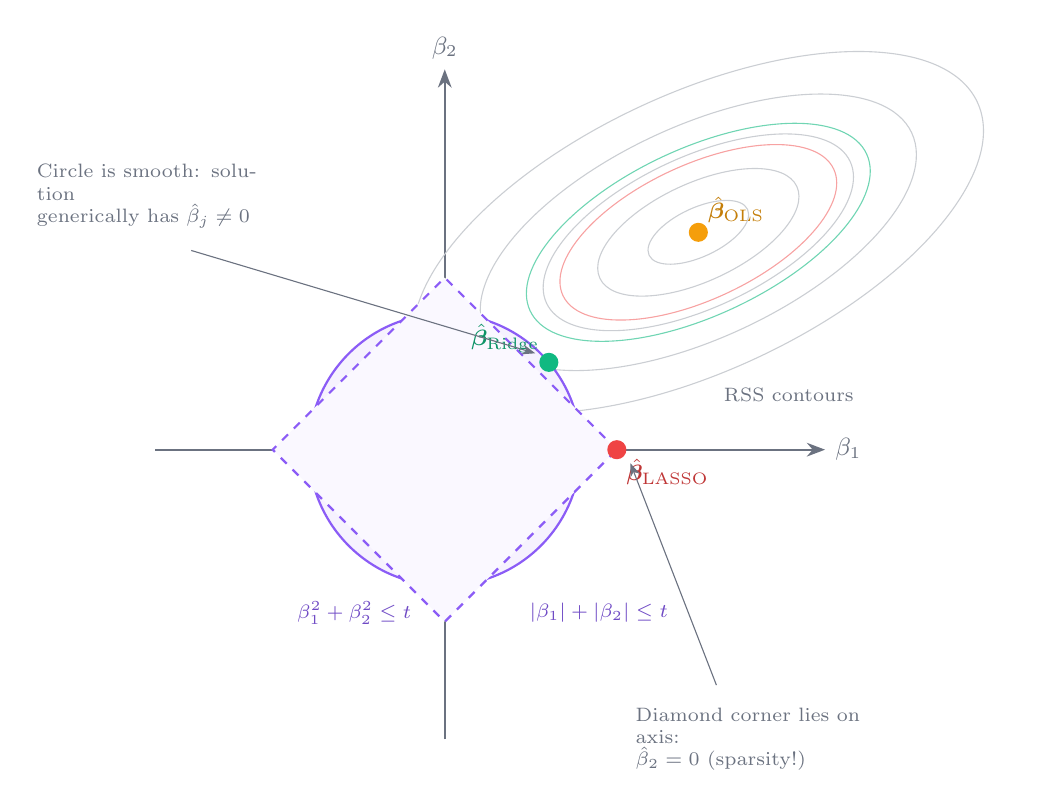
\begin{tikzpicture}[>=Stealth, scale=1.15]

  % --- Axes ---
  \draw[->, secondary, thick] (-3.2,0) -- (4.2,0) node[right, font=\small] {$\beta_1$};
  \draw[->, secondary, thick] (0,-3.2) -- (0,4.2) node[above, font=\small] {$\beta_2$};

  % --- OLS solution ---
  \coordinate (ols) at (2.8,2.4);
  \fill[response] (ols) circle (3pt);
  \node[above right, response!80!black, font=\footnotesize\bfseries] at (ols)
    {$\hat{\bm{\beta}}_{\mathrm{OLS}}$};

  % --- RSS contour ellipses (centered on OLS, tilted) ---
  \foreach \r in {0.6, 1.2, 1.85, 2.6, 3.4} {
    \draw[secondary!35, thin, rotate around={25:(ols)}]
      (ols) ellipse ({\r} and {\r*0.45});
  }
  \node[secondary, font=\scriptsize] at (3.8,0.6) {RSS contours};

  % --- L2 constraint region (circle) ---
  \draw[constraint, thick, fill=constraint!8] (0,0) circle (1.5);
  \node[constraint!80!black, font=\scriptsize] at (-1.0,-1.8)
    {$\beta_1^2+\beta_2^2 \le t$};

  % --- L1 constraint region (diamond) ---
  \draw[constraint, thick, dashed, fill=constraint!4]
    (1.9,0) -- (0,1.9) -- (-1.9,0) -- (0,-1.9) -- cycle;
  \node[constraint!80!black, font=\scriptsize] at (1.7,-1.8)
    {$|\beta_1|+|\beta_2| \le t$};

  % --- Ridge solution (ellipse tangent to circle) ---
  \coordinate (ridge) at ({1.5*cos(40)},{1.5*sin(40)});
  \fill[projection] (ridge) circle (3pt);
  \node[above left, projection!80!black, font=\footnotesize\bfseries] at (ridge)
    {$\hat{\bm{\beta}}_{\mathrm{Ridge}}$};
  % Ridge ellipse (approximate tangent)
  \draw[projection!60, thin, rotate around={25:(ols)}]
    (ols) ellipse ({2.05} and {2.05*0.45});

  % --- LASSO solution (ellipse tangent to diamond corner) ---
  \coordinate (lasso) at (1.9,0);
  \fill[residual] (lasso) circle (3pt);
  \node[below right, residual!80!black, font=\footnotesize\bfseries] at (lasso)
    {$\hat{\bm{\beta}}_{\mathrm{LASSO}}$};
  % LASSO ellipse (approximate tangent at corner)
  \draw[residual!50, thin, rotate around={25:(ols)}]
    (ols) ellipse ({1.65} and {1.65*0.45});

  % --- Annotation: why corners produce zeros ---
  \draw[->, secondary, thin] (3.0,-2.6) -- ($(lasso)+(0.15,-0.15)$);
  \node[secondary, font=\scriptsize, align=left, text width=3.2cm] at (3.5,-3.2)
    {Diamond corner lies on axis:\\$\hat\beta_2 = 0$ (sparsity!)};

  % --- Annotation: circle has no corners ---
  \draw[->, secondary, thin] (-2.8,2.2) -- ($(ridge)+(-0.15,0.1)$);
  \node[secondary, font=\scriptsize, align=left, text width=3cm] at (-3.2,2.8)
    {Circle is smooth: solution\\generically has $\hat\beta_j\neq 0$};

\end{tikzpicture}
\caption{Ridge vs.\ LASSO constraint regions.  The OLS
estimate~$\hat{\bm{\beta}}_{\mathrm{OLS}}$ (amber dot) sits at the
centre of the elliptical RSS contours.  Regularisation constrains the
solution to lie within a region around the origin.  \textbf{Ridge}
(solid circle, $L^2$) shrinks all coefficients smoothly toward zero.
\textbf{LASSO} (dashed diamond, $L^1$) has \emph{corners} on the
coordinate axes; the first contour ellipse to touch the diamond
typically hits a corner, setting some coefficients exactly to zero
and producing a sparse model.}
\label{fig:ridge-lasso}
\end{figure}


%----------------------------------------------------------------------
\subsection{Reconnecting to the geometric framework}
%----------------------------------------------------------------------

Neither Ridge nor LASSO is an orthogonal projection.
Both sacrifice the ``closest point'' property---accepting bias---in
exchange for a (potentially large) reduction in variance.
The telescope analogy captures the trade-off:
you give up perfect aim to eliminate the shake.

Yet the connection to the projection framework runs deeper than it
first appears.
Recall from Section~\ref{sec:multicollinearity} that
multicollinearity makes the column space geometrically thin:
the eigenvalue spectrum of $\bX^\top\bX$ has a few large values
and some dangerously small ones.
OLS faithfully projects onto this flattened space, and in doing so
amplifies noise along the thin directions.
Ridge responds by \emph{reshaping} the eigenvalue landscape:
it replaces $\lambda_k$ with $\lambda_k + \lambda$, inflating every
eigenvalue and rounding out the column space's geometry.
The thinner a direction was, the more it gets inflated in relative
terms---precisely the directions that needed stabilising.

Ridge is the projection framework's answer to its own weakness.
When the geometry is unstable, you reshape the geometry.


%--- Gaussian prerequisite ---

\medskip
\begin{remark}[Prerequisite: where the Gaussian enters]
Everything up to this point has been \emph{purely geometric}---no
distributional assumptions were needed.
The Projection Theorem, the hat matrix properties, Pythagoras, FWL,
leverage, influence, multicollinearity, OVB, and even regularisation
all follow from linear algebra alone.

To perform \emph{inference}---hypothesis tests, $p$-values, confidence
intervals---we need a probability model.
The standard assumption is:
\[
  \by = \bX\bm{\beta} + \bm{\varepsilon},
  \qquad
  \bm{\varepsilon} \sim \mathcal{N}(\bm{0},\, \sigma^2 \bI_n).
\]
That is, the errors are independent, identically distributed, and
Gaussian (normally distributed).

Why does the Gaussian matter?
\begin{itemize}[nosep]
  \item \textbf{Exactness:} Under Gaussianity, $\bhat$ is exactly
        $\mathcal{N}(\bm{\beta},\, \sigma^2(\bX^\top\bX)^{-1})$---not
        just approximately. This gives us exact $t$- and $F$-distributions
        for test statistics, valid in any sample size.
  \item \textbf{Without Gaussianity:} The Central Limit Theorem still
        ensures that $\bhat$ is \emph{approximately} normal in large samples.
        So inference is approximately valid even when the true error
        distribution is non-Gaussian---but only asymptotically.
  \item \textbf{Geometry of the Gaussian:} A Gaussian vector projected
        onto a subspace remains Gaussian. This is why the hat matrix
        preserves normality: $\yhat = \bH\by$ and
        $\be = \bM\by$ are both Gaussian, and they are
        \emph{independent} (because $\bH\bM = \bm{0}$).
        Independence of $\yhat$ and $\be$ is what makes the $F$-test work.
\end{itemize}
The next section uses these distributional facts to build hypothesis tests.
\end{remark}

\medskip
\noindent\textit{Regularisation reshapes the geometry to stabilise
estimates, but it cannot tell us whether the extra predictors are
\emph{statistically significant}.
For that, we need to compare two projections---one with and one
without the extra variables---and ask whether the improvement is
larger than what noise alone would produce.
This brings us to the $F$-test.}


%======================================================================
\section{Testing with Geometry: The $F$-Test}\label{sec:ftest}
%======================================================================

\subsection{Comparing two projections}

Consider two nested models:
\begin{itemize}[nosep]
  \item \textbf{Restricted:} $\by = \bX_R\bm{\beta}_R + \be_R$,
        with column space $\Col(\bX_R)$.
  \item \textbf{Unrestricted:} $\by = \bX\bm{\beta} + \be$,
        with column space $\Col(\bX)\supseteq\Col(\bX_R)$.
\end{itemize}
Both models project $\by$ onto their respective column spaces.
The restricted projection $\yhat_R$ and the unrestricted projection
$\yhat$ satisfy $\norm{\be_R}\ge\norm{\be}$ (by Proposition~\ref{prop:r2mono}).
The gap $\yhat - \yhat_R$ lies in $\Col(\bX)$ and is perpendicular to
$\Col(\bX_R)$.

\subsection{The $F$-statistic}

\begin{definition}
The $F$-statistic for testing $H_0$: the $q$ extra predictors
have zero coefficients is
\begin{equation}\label{eq:fstat}
  F = \frac{(\text{SSE}_R - \text{SSE})/q}{\text{SSE}/(n-p)}
    = \frac{\norm{\yhat-\yhat_R}^2/q}{\norm{\be}^2/(n-p)}.
\end{equation}
Under $H_0$ and standard Gaussian assumptions,
$F\sim F_{q,\,n-p}$.
\end{definition}

\begin{keyinsight}
The $F$-test measures whether the \emph{distance between two projections}
is surprisingly large relative to the residual noise.
The numerator is the squared length of the gap between projections,
normalised by the number of extra dimensions ($q$).
The denominator is the residual noise level.
If $F\approx 1$, the extra predictors captured only noise.
If $F\gg 1$, they captured real signal.
\end{keyinsight}

% --- Figure 6: F-test gap between projections ---

\begin{figure}[ht]
\centering
\tdplotsetmaincoords{62}{125}
\begin{tikzpicture}[tdplot_main_coords, scale=1.5, >=Stealth]

  % --- Full plane Col(X) ---
  \fill[colspace!10] (-3,-2.5,0) -- (3.2,-2.5,0) -- (3.2,2.5,0) -- (-3,2.5,0) -- cycle;
  \draw[colspace!30, line width=0.4pt]
    (-3,-2.5,0) -- (3.2,-2.5,0) -- (3.2,2.5,0) -- (-3,2.5,0) -- cycle;
  \node[colspace!70!black, font=\scriptsize\itshape] at (2.7,-2.0,0)
    {$\operatorname{Col}(\bm{X})$};

  % --- Restricted subspace Col(X_R) as a line in the plane ---
  \draw[constraint!70, very thick] (-2.8,-0.56,0) -- (2.8,0.56,0);
  \node[constraint!80!black, font=\scriptsize\itshape] at (2.9,0.9,0)
    {$\operatorname{Col}(\bm{X}_R)$};

  % Origin
  \fill[secondary] (0,0,0) circle (1.2pt);
  \node[below left, secondary, font=\scriptsize] at (0,0,0) {$\bm{0}$};

  % --- y above the plane ---
  \coordinate (y) at (1.6,1.4,2.6);
  \draw[->, response, very thick] (0,0,0) -- (y)
    node[above right, font=\footnotesize\bfseries] {$\bm{y}$};

  % --- yhat: projection onto full Col(X) ---
  \coordinate (yhat) at (1.6,1.4,0);
  \draw[->, projection, very thick] (0,0,0) -- (yhat)
    node[below right=1pt, font=\footnotesize\bfseries] {$\hat{\bm{y}}$};

  % --- yhatR: projection onto Col(X_R) (on the line) ---
  \coordinate (yhatR) at (1.75,0.35,0);
  \draw[->, constraint, thick] (0,0,0) -- (yhatR)
    node[below=3pt, font=\footnotesize\bfseries] {$\hat{\bm{y}}_R$};

  % --- Residual e = y - yhat (perpendicular to plane, going up) ---
  \draw[->, residual, thick, dashed] (yhat) -- (y);
  \node[right=3pt, residual!80!black, font=\footnotesize] at ($(yhat)!0.5!(y)$)
    {$\bm{e}=\bm{y}-\hat{\bm{y}}$};

  % --- Gap: yhat - yhatR (in the plane, perp to Col(X_R)) ---
  \draw[->, response!80!black, thick] (yhatR) -- (yhat);
  \node[above=3pt, response!80!black, font=\footnotesize] at ($(yhatR)!0.5!(yhat)$)
    {$\hat{\bm{y}}-\hat{\bm{y}}_R$};

  % --- Right angle 1: e perpendicular to plane at yhat ---
  \draw[secondary, line width=0.5pt]
    ($(yhat)+(-0.16,0,0)$) -- ($(yhat)+(-0.16,0,0.16)$) -- ($(yhat)+(0,0,0.16)$);

  % --- Right angle 2: gap perpendicular to Col(X_R) at yhatR ---
  \pgfmathsetmacro{\ux}{0.98}
  \pgfmathsetmacro{\uy}{0.196}
  \pgfmathsetmacro{\vx}{-0.196}
  \pgfmathsetmacro{\vy}{0.98}
  \draw[secondary, line width=0.5pt]
    ($(yhatR)+0.14*(\ux,\uy,0)$)
    -- ($(yhatR)+0.14*(\ux,\uy,0)+0.14*(\vx,\vy,0)$)
    -- ($(yhatR)+0.14*(\vx,\vy,0)$);

  % --- Right angle 3: (yhat - yhatR) perpendicular to e ---
  \draw[secondary, line width=0.5pt]
    ($(yhat)+(0,-0.16,0)$) -- ($(yhat)+(0,-0.16,0.16)$) -- ($(yhat)+(0,0,0.16)$);

  % --- F-statistic annotation ---
  \draw[decorate, decoration={brace, amplitude=4pt, mirror},
    secondary, thick]
    ($(yhatR)+(0.2,-0.15,0)$) -- ($(yhat)+(0.2,-0.15,0)$);
  \node[secondary, font=\scriptsize, right, align=left] at (2.4,0.2,0)
    {$\|\hat{\bm{y}}-\hat{\bm{y}}_R\|^2/(p-q)$\\[2pt]
     $F$-numerator};

  \draw[decorate, decoration={brace, amplitude=4pt},
    secondary, thick]
    ($(yhat)+(0.35,0,0)$) -- ($(y)+(0.35,0,0)$);
  \node[secondary, font=\scriptsize, right, align=left] at (2.3,0.7,1.3)
    {$\|\bm{e}\|^2/(n-p)$\\[2pt]
     $F$-denominator};

\end{tikzpicture}
\caption{The $F$-test as the gap between two projections.
$\hat{\bm{y}}_R$ is the projection of~$\bm{y}$ onto the restricted
subspace $\operatorname{Col}(\bm{X}_R)$ (a line), and $\hat{\bm{y}}$ is
the projection onto the full $\operatorname{Col}(\bm{X})$ (a plane
containing the line).  The three segments are mutually perpendicular by
the Pythagorean theorem:
$\|\bm{y}-\hat{\bm{y}}_R\|^2 =
 \|\hat{\bm{y}}-\hat{\bm{y}}_R\|^2 + \|\bm{e}\|^2$.
The $F$-statistic compares the ``explained gap''
$\|\hat{\bm{y}}-\hat{\bm{y}}_R\|^2$ (what the extra predictors bought)
to the residual $\|\bm{e}\|^2$ (what remains unexplained), each
normalised by its degrees of freedom.}
\label{fig:f-test}
\end{figure}

\begin{remark}
When $q=1$ (testing a single coefficient), $F = t^2$ where $t$ is the
usual $t$-statistic.
The $t$-test is the $F$-test in one dimension.
\end{remark}

\subsection{Confidence ellipsoids}

The sampling distribution of $\bhat$ is
$\bhat\sim\mathcal{N}(\bm{\beta},\;\sigma^2(\bX^\top\bX)^{-1})$.
A $(1-\alpha)$-confidence ellipsoid for $\bm{\beta}$ is
\[
  \bigl\{\bm{b}\in\R^p :
  (\bhat-\bm{b})^\top(\bX^\top\bX)(\bhat-\bm{b})
  \le p\,s^2\,F_{p,n-p,\alpha}
  \bigr\}.
\]
The ellipsoid's axes align with the eigenvectors of $\bX^\top\bX$
and its semi-axis lengths are proportional to $1/\sqrt{\lambda_k}$.
Directions where the column space is ``thin'' (small $\lambda_k$)
produce long axes---more uncertainty.
This is the same eigenvalue structure that drives multicollinearity
and Ridge shrinkage: everything connects.

\medskip
\noindent\textit{The $F$-test and confidence ellipsoids complete our
inferential toolkit.
But before we summarise, it is worth stepping back and asking:
where does the geometric framework \emph{break down}?
What can projections not tell us, and where must we look beyond
linear algebra for answers?}


%======================================================================
\section{The Limits of the Geometric Framework}\label{sec:limits}
%======================================================================

The Projection Theorem is powerful but not omniscient.
Three fundamental limitations bound the geometric framework, and
intellectual honesty demands that we name them clearly.

\subsection{Causality: the geometry cannot choose the wall}

The geometry tells you \emph{how well} you are projecting.
It cannot tell you \emph{whether you are projecting onto the right wall}.
Omitted variable bias (\S\ref{sec:failures}) is invisible to every
geometric diagnostic: the residuals are still perpendicular, $R^2$ still
decomposes via Pythagoras, the hat matrix is still idempotent.
The Scoreboard reads green for a perfectly projected regression on the
wrong column space.

To choose the right wall, you need \emph{causal reasoning}: directed
acyclic graphs, potential outcomes, natural experiments, instrumental
variables. These are structural tools, not geometric ones.
No amount of staring at shadows will tell you whether the flashlight
is aimed at the right surface.

\subsection{The inner product: whose notion of ``closest''?}

Everything in these notes assumed the Euclidean inner product---all
observations weighted equally, all errors independent.
If observations have \textbf{heteroscedastic} errors
($\text{Var}(\varepsilon_i) = \sigma_i^2$) or are
\textbf{autocorrelated},
the inner product is wrong.
The ``perpendicular'' is not truly perpendicular in the correct metric,
and the ``closest point'' is not truly closest.

\textbf{Generalised Least Squares (GLS)} fixes this by replacing the
Euclidean inner product $\ip{\bm{u}}{\bm{v}}=\bm{u}^\top\bm{v}$ with
$\ip{\bm{u}}{\bm{v}}_\Omega = \bm{u}^\top\bm{\Omega}^{-1}\bm{v}$,
where $\bm{\Omega} = \text{Var}(\bm{\varepsilon})$.
The Projection Theorem still applies, but in a different geometry---a
tilted space where ``perpendicular'' has a new meaning:
\[
  \bhat_{\text{GLS}}
  = (\bX^\top\bm{\Omega}^{-1}\bX)^{-1}\bX^\top\bm{\Omega}^{-1}\by.
\]
The moral: the geometry generalises, but only if you choose the right
inner product.

\subsection{Linearity: the column space is flat}

The column space is \emph{flat}---a hyperplane through the origin.
If the true relationship is curved, the best flat projection may be
a poor representation, like pressing a globe onto a table.
Polynomial features enlarge the column space to include some curvature,
but the bias-variance trade-off (Notebook~3's overfitting trap) limits
how far this can go.
Kernel methods, trees, and neural networks define curved ``column
spaces''---function spaces that lie beyond the reach of linear
projection geometry.

The Projection Theorem is not wrong in these settings.  It is simply
not enough.


%======================================================================
\section{Summary: The Geometric Rosetta Stone}\label{sec:rosetta}
%======================================================================

\subsection*{Closing the circle}

In 1801, Carl Friedrich Gauss took 41 noisy astronomical observations and
dropped a perpendicular from them onto the subspace of Keplerian orbits.
The shadow---the nearest point on that subspace---told him where to
point the telescope.  On New Year's Eve, von~Zach found Ceres within
half a degree of the predicted position.

Every time you call \texttt{lm()} in R or
\texttt{sklearn.LinearRegression().fit()} in Python, you perform
the same act that Gauss performed: you cast a shadow of noisy data
onto a subspace of possible fitted values, you measure the
perpendicular gap that remains, and you trust the right angle.

The mathematics has not changed in two centuries.  Only the notation
is different.

\subsection*{The Rosetta Stone}

Every concept in OLS regression has a geometric face and an algebraic
face.  Table~\ref{tab:rosetta} provides the complete correspondence.
Where the Pythagorean decomposition and $R^2$ require demeaned vectors,
this is noted explicitly.

\begin{table}[ht]
\centering
\caption{The Geometric Rosetta Stone.}\label{tab:rosetta}
\small
\begin{tabular}{@{}lll@{}}
\toprule
\textbf{Statistical concept} & \textbf{Geometric interpretation} & \textbf{Formula / characterisation} \\
\midrule
\multicolumn{3}{@{}l}{\textit{Core projection}} \\[2pt]
Fitted values $\yhat$ & Shadow on the wall & $\bH\by$ \\
Residuals $\be$ & Perpendicular gap & $(\bI-\bH)\by$ \\
Coefficients $\bhat$ & Coordinates of the shadow & $(\bX^\top\bX)^{-1}\bX^\top\by$ \\
Normal equations & Orthogonality condition & $\bX^\top\be=\bm{0}$ \\
Intercept $\hat{\beta}_0$ & Ensures $\bar{e}=0$; centres the & $\bm{1}\in\Col(\bX)$ guarantees \\
 & projection around the data mean & $\be\perp\bm{1}$ \\[4pt]
\midrule
\multicolumn{3}{@{}l}{\textit{Decomposition and fit quality (demeaned vectors $\tilde{\by}=\by-\bar{y}\bm{1}$, $\tilde{\yhat}=\yhat-\bar{y}\bm{1}$)}} \\[2pt]
SST $=$ SSR $+$ SSE & Pythagorean theorem & $\norm{\tilde{\by}}^2=\norm{\tilde{\yhat}}^2+\norm{\be}^2$ \\
$R^2$ & Squared cosine of angle & $\cos^2\theta = \norm{\tilde{\yhat}}^2/\norm{\tilde{\by}}^2$ \\
Degrees of freedom & Dimension of the residual & $\dim\bigl(\Col(\bX)^\perp\bigr) = n-p$ \\
 & subspace & \\
Adjusted $R^2$ & $R^2$ corrected for dimension & $1 - \frac{\norm{\be}^2/(n-p)}{\norm{\tilde{\by}}^2/(n-1)}$ \\[4pt]
\midrule
\multicolumn{3}{@{}l}{\textit{Projection operators and diagnostics}} \\[2pt]
Hat matrix $\bH$ & Projection operator & $\bH^2=\bH,\;\bH^\top=\bH$ \\
Leverage $h_{ii}$ & Arm length in column space & $\diag(\bH)$ \\
Cook's distance $D_i$ & Arm length $\times$ surprise & $\propto h_{ii}\cdot e_i^2$ \\
Gauss--Markov (BLUE) & Closest point in subspace & Projection Theorem \\[4pt]
\midrule
\multicolumn{3}{@{}l}{\textit{Structure and partial effects}} \\[2pt]
FWL theorem & Sequential orthogonal projections & $\bhat_2 = (\bX_2^\top\bM_1\bX_2)^{-1}\bX_2^\top\bM_1\by$ \\
Multicollinearity & Thin, nearly degenerate column space & $\kappa(\bX^\top\bX)\gg 1$ \\
OVB & Wrong column space & $\text{Bias} = \bm{\Gamma}\bm{\beta}_2$ \\[4pt]
\midrule
\multicolumn{3}{@{}l}{\textit{Regularisation (constrained optimisation: trading bias for stability)}} \\[2pt]
Ridge ($L^2$) & Constrained optimisation within a sphere; & Shrinks unstable eigenvector \\
 & trades bias for variance reduction & directions: $\lambda_k/(\lambda_k+\lambda)$ \\
LASSO ($L^1$) & Constrained optimisation within a diamond; & Corner solutions $\Rightarrow$ exact zeros \\
 & trades bias for sparsity & $\Rightarrow$ automatic variable selection \\[4pt]
\midrule
\multicolumn{3}{@{}l}{\textit{Inference}} \\[2pt]
$F$-test & Gap between two projections & $F = \frac{\norm{\yhat-\yhat_R}^2/q}{\norm{\be}^2/(n-p)}$ \\
Confidence ellipsoid & Region of plausible shadows & Axes $\propto 1/\sqrt{\lambda_k}$ \\
\bottomrule
\end{tabular}
\end{table}

\subsection*{The story in sixteen lines}

\begin{center}
\fbox{\parbox{0.88\textwidth}{\centering\itshape
Regression is a projection.\\
Coefficients are coordinates of the shadow.\\
The residual is perpendicular to the column space.\\
The intercept guarantees the residuals have mean zero.\\
$R^2$ is the squared cosine of an angle between demeaned vectors.\\
Variance decomposition is Pythagoras applied to a right triangle.\\
Degrees of freedom count the dimensions the residual can roam.\\
Gauss--Markov says: no linear unbiased estimator gets closer.\\
Controlling for a variable means projecting it away first.\\
Leverage measures how far each point reaches into the column space.\\
Influence is leverage times surprise.\\
Multicollinearity flattens the column space to a sliver.\\
Omitted variables tilt the column space to the wrong wall.\\
The $F$-test measures the gap between two nested projections.\\
Ridge and LASSO trade bias for stability---they are not projections.\\
And geometry alone cannot tell you which wall to aim at.
}}
\end{center}

\bigskip

\noindent
Gauss pointed a pencil at the sky and found an asteroid.  You point a
line of code at a dataset and find a pattern.  In both cases, the
method is the same: drop a perpendicular, read the shadow, respect the
right angle.

\medskip

\noindent
The geometry was always there, hiding inside every formula you
memorised and every $p$-value you reported.  These notes did not
create it.  They just turned on the light.

%======================================================================
% References
%======================================================================

\bigskip
\noindent\textbf{Further reading.}
\begin{itemize}[nosep]
  \item S.\,M.\ Stigler, \emph{The History of Statistics: The Measurement of
        Uncertainty before 1900}, Harvard University Press, 1986.
        \textit{Chapter~4 gives a superb account of Gauss, Ceres, and the
        birth of least squares.}
  \item G.\,W.\ Dunnington, \emph{Gauss: Titan of Science}, Mathematical
        Association of America, 2004 (reprint).
        \textit{The definitive biography; see chapters on the Ceres
        prediction and the development of the method of least squares.}
  \item G.\,A.\,F.\ Seber, \emph{Linear Regression Analysis}, Wiley, 1977.
  \item R.\ Davidson and J.\,G.\ MacKinnon, \emph{Estimation and Inference
        in Econometrics}, Oxford University Press, 1993.
  \item R.\ Christensen, \emph{Plane Answers to Complex Questions: The Theory
        of Linear Models}, 4th ed., Springer, 2011.
  \item S.\ Weisberg, \emph{Applied Linear Regression}, 4th ed., Wiley, 2014.
\end{itemize}


%======================================================================
\appendix
\section{Proofs for the Mathematically Curious}\label{app:proofs}
%======================================================================

These proofs are included for completeness and for readers who want
to verify the foundations. They are not required for following the
main narrative.


%----------------------------------------------------------------------
\subsection{Proof of the Projection Theorem (Theorem~\ref{thm:projection})}
%----------------------------------------------------------------------

\begin{proof}
We work in $V = \R^n$ with the Euclidean inner product, and $S$ is a
$p$-dimensional subspace (hence closed).  The proof has three parts:
existence, uniqueness, and the orthogonality characterisation.

\medskip
\noindent\textbf{Step 1: Existence.}
Let $d = \inf_{\bm{s}\in S}\norm{\by - \bm{s}}$.
Choose any $\bm{s}_0 \in S$. Then every minimising candidate satisfies
$\norm{\by - \bm{s}} \le \norm{\by - \bm{s}_0}$,
so the search is confined to the closed, bounded set
$\{\bm{s}\in S : \norm{\by - \bm{s}} \le \norm{\by - \bm{s}_0}\}$.
Since $S$ is a subspace of a finite-dimensional space, this set is compact.
The continuous function $\bm{s}\mapsto\norm{\by - \bm{s}}$ attains its
minimum on a compact set, so there exists $\yhat\in S$ with
$\norm{\by - \yhat} = d$.

\medskip
\noindent\textbf{Step 2: Uniqueness.}
Suppose $\yhat$ and $\yhat'$ are both minimisers.
By the parallelogram law,
\[
  \norm{(\by - \yhat) + (\by - \yhat')}^2
  + \norm{(\by - \yhat) - (\by - \yhat')}^2
  = 2\norm{\by - \yhat}^2 + 2\norm{\by - \yhat'}^2.
\]
The left-hand side rewrites as
$\norm{2\by - \yhat - \yhat'}^2 + \norm{\yhat' - \yhat}^2$,
and the right-hand side equals $4d^2$.
Now $\frac{1}{2}(\yhat + \yhat') \in S$ (since $S$ is a subspace), so
\[
  \norm{2\by - \yhat - \yhat'}^2
  = 4\,\norm{\by - \tfrac{\yhat+\yhat'}{2}}^2
  \ge 4d^2.
\]
Therefore $\norm{\yhat' - \yhat}^2 \le 4d^2 - 4d^2 = 0$,
which forces $\yhat' = \yhat$.

\medskip
\noindent\textbf{Step 3: Orthogonality condition.}
Let $\bm{v}\in S$ be arbitrary and $t\in\R$.
Since $\yhat + t\bm{v}\in S$, the minimality of $\yhat$ gives
\[
  f(t)
  \;=\; \norm{\by - \yhat - t\bm{v}}^2
  \;=\; \norm{\by - \yhat}^2
        - 2t\,\ip{\by - \yhat}{\bm{v}}
        + t^2\norm{\bm{v}}^2
  \;\ge\; f(0)
  \quad\text{for all } t\in\R.
\]
The function $f$ is a quadratic in $t$ with minimum at $t=0$.
Setting $f'(0) = 0$:
\[
  f'(0) = -2\,\ip{\by-\yhat}{\bm{v}} = 0
  \qquad\Longrightarrow\qquad
  \ip{\by - \yhat}{\bm{v}} = 0.
\]
Since $\bm{v}\in S$ was arbitrary, $(\by - \yhat)\perp S$.

\medskip
\noindent\textbf{Conversely}, if $\yhat\in S$ satisfies $(\by-\yhat)\perp S$,
then for any $\bm{s}\in S$:
\[
  \norm{\by - \bm{s}}^2
  = \norm{(\by - \yhat) + (\yhat - \bm{s})}^2
  = \norm{\by - \yhat}^2 + \norm{\yhat - \bm{s}}^2
  \ge \norm{\by - \yhat}^2,
\]
where the cross term vanishes because $(\by - \yhat)\perp(\yhat-\bm{s})$
(since $\yhat - \bm{s}\in S$), and the Pythagorean theorem applies.
Hence $\yhat$ is the unique minimiser.
\end{proof}


%----------------------------------------------------------------------
\subsection{Characterisation of Orthogonal Projections (Theorem~\ref{thm:proj-char})}
%----------------------------------------------------------------------

\begin{theorem}[Characterisation of Orthogonal Projections]\label{thm:proj-char}
Let $\bm{P}\in\R^{n\times n}$.  The following are equivalent:
\begin{enumerate}[nosep,label=(\alph*)]
  \item $\bm{P}$ is the matrix of orthogonal projection onto $\Col(\bm{P})$.
  \item $\bm{P}^2 = \bm{P}$ and $\bm{P}^\top = \bm{P}$.
\end{enumerate}
\end{theorem}

\begin{proof}
\textbf{(a) $\Rightarrow$ (b).}
Let $W = \Col(\bm{P})$ and suppose $\bm{P}$ is the orthogonal projection
onto $W$.  For any $\bm{v}\in\R^n$, $\bm{P}\bm{v}\in W$ and
$\bm{v} - \bm{P}\bm{v}\in W^\perp$.

\emph{Idempotency:}
Since $\bm{P}\bm{v}\in W$, projecting it again gives
$\bm{P}(\bm{P}\bm{v}) = \bm{P}\bm{v}$. Hence $\bm{P}^2 = \bm{P}$.

\emph{Symmetry:}
For any $\bm{u}, \bm{v}\in\R^n$,
\begin{align*}
  \ip{\bm{P}\bm{u}}{\bm{v}}
  &= \ip{\bm{P}\bm{u}}{\bm{P}\bm{v} + (\bm{v}-\bm{P}\bm{v})} \\
  &= \ip{\bm{P}\bm{u}}{\bm{P}\bm{v}} + \ip{\bm{P}\bm{u}}{\bm{v}-\bm{P}\bm{v}} \\
  &= \ip{\bm{P}\bm{u}}{\bm{P}\bm{v}},
\end{align*}
because $\bm{P}\bm{u}\in W$ and $\bm{v}-\bm{P}\bm{v}\in W^\perp$.
By the same argument with roles swapped,
$\ip{\bm{u}}{\bm{P}\bm{v}} = \ip{\bm{P}\bm{u}}{\bm{P}\bm{v}}$.
Therefore $\ip{\bm{P}\bm{u}}{\bm{v}} = \ip{\bm{u}}{\bm{P}\bm{v}}$ for all
$\bm{u},\bm{v}$, which means $\bm{P}^\top = \bm{P}$.

\medskip
\noindent\textbf{(b) $\Rightarrow$ (a).}
Assume $\bm{P}^2 = \bm{P}$ and $\bm{P}^\top = \bm{P}$.
Let $W = \Col(\bm{P})$.
We must show: for every $\bm{v}\in\R^n$,
(i) $\bm{P}\bm{v}\in W$, and
(ii) $\bm{v} - \bm{P}\bm{v} \perp W$.

Part (i) is immediate: $\bm{P}\bm{v}$ is a column of $\bm{P}$ (times scalars),
hence in $\Col(\bm{P}) = W$.

For part (ii), let $\bm{w}\in W$ be arbitrary. Then $\bm{w} = \bm{P}\bm{z}$
for some $\bm{z}$.  Compute:
\[
  \ip{\bm{v} - \bm{P}\bm{v}}{\bm{w}}
  = \ip{\bm{v} - \bm{P}\bm{v}}{\bm{P}\bm{z}}
  = (\bm{v} - \bm{P}\bm{v})^\top\bm{P}\bm{z}
  = \bm{v}^\top\bm{P}\bm{z} - \bm{v}^\top\bm{P}^\top\bm{P}\bm{z}.
\]
Using $\bm{P}^\top = \bm{P}$ and then $\bm{P}^2 = \bm{P}$:
\[
  = \bm{v}^\top\bm{P}\bm{z} - \bm{v}^\top\bm{P}^2\bm{z}
  = \bm{v}^\top\bm{P}\bm{z} - \bm{v}^\top\bm{P}\bm{z}
  = 0.
\]
Since $\bm{w}\in W$ was arbitrary, $(\bm{v}-\bm{P}\bm{v})\perp W$.
\end{proof}


%----------------------------------------------------------------------
\subsection{Proof that $h_{ii} \ge 1/n$ when an intercept is present (Remark~\ref{rem:hii-intercept})}
%----------------------------------------------------------------------

When the model includes an intercept, $\bm{1}\in\Col(\bX)$, so
$\bH\bm{1} = \bm{1}$. The $i$-th row of $\bH$ therefore sums to~1:
$\sum_{j=1}^n h_{ij} = 1$.

Since $\bH$ is an orthogonal projection, $h_{ij}^2 \le h_{ii}\cdot h_{jj} \le h_{ii}$
(by Cauchy--Schwarz applied to the rows/columns of $\bH$).  In particular,
\[
  1 = \Bigl(\sum_{j=1}^n h_{ij}\Bigr)^2
  \le n\sum_{j=1}^n h_{ij}^2
  = n\,(\bH^2)_{ii}
  = n\,h_{ii},
\]
where the inequality is Cauchy--Schwarz (applied to the sum $\sum_j h_{ij}\cdot 1$)
and the last step uses $\bH^2 = \bH$.
Therefore $h_{ii}\ge 1/n$.

Without an intercept, it is possible to have $h_{ii} = 0$ (for an observation
$\bm{x}_i$ orthogonal to every column of $\bX$), so the general bound is
$0 \le h_{ii} \le 1$.


\end{document}
